
\chapter{Search Strategy}
\label{ch:SearchStrategy}
%Deep thoughts go here.
This chapter will describe the major backgrounds and outline a search strategy used in the analysis.  The kinematic regions for the signal will be defined as well as the introduction of neural networks to assist with the separation of signal and background like events.  This chapter contains material coauthored with the ATLAS Collaboration.  I developed the signal samples and analysis framework, optimized the signal regions, and was responsible for the the background modeling in the regions shown here including the fake rate studies.  Other members of the ATLAS Collaboration developed the background samples used to produce the results presented in this chapter.


\section{Major Backgrounds}
There are a large number of Standard Model processes that can end up in the signal region and share a similar final state topology as the studied signal process, $t\bar{t}\rightarrow b l \nu q \gamma$.  All of these processes are modeled with Monte Carlo (MC) simulation, with the exception of particles that fake other particles (leptons and photons) which are done using data-driven techniques because they are poorly modeled with MC.  A full list of the Monte Carlo samples used for each background can be found in Appendix \ref{app:MC_Samples}. 

The dominant backgrounds in this search are Standard Model $t\bar{t}$, Standard Model $t\bar{t}+\gamma$, as well as W+jets and W+jets with an associated photon (W+jets+$\gamma$).  These along with minor backgrounds (Standard Model single top events, Z+jets (Z+jets+$\gamma$), $t\bar{t}$+Vector Boson, diboson) are all modeled with MC and some data-driven estimates and corrections are applied.  The various backgrounds modeled in this search are summarized here:

\begin{description}
\item[\textbf{SM Processes}:]  SM $t\bar{t}$, W+jets, Z+jets, single top, diboson, $t\bar{t}$+V are modeled with MC simulations.  Control and validation regions are designed to test preformance of the largest of these background proceses, $t\bar{t}$ and W+jets.  A discussion of the modeling of the major SM processes without photons and a derivation of additional scale factors for these processes is shown in Section \ref{sec:BKGnoPho}.

\item[\textbf{SM Processes with an associated photon}:] SM + associated photon processes: $t\bar{t}+\gamma$, W+jets+$\gamma$, Z+jets+$\gamma$ are modeled with MC simulation and overlap removal is applied to the SM processes to remove events with similar phase spaces since these processes are a subset of the SM process.  MC simulations are created with additional statistics for these processes.  Further details are presented in Section \ref{sec:BKGPho}.

\item[\textbf{Fake Leptons}:] Non-prompt or fake electrons and muons can arise from semi-leptonic decay of $b$ and $c$ quarks.  For electrons additional contributions from photon conversions and jets in the electromagnetic calorimeter can lead to lepton fakes.  Muons can be faked via energetic showers in the hadronic calorimeter or from hadrons that punch through the hadronic calorimeter.  The matrix method is used to estimate the number of events with fake leptons as described in Section \ref{sec:FakeLep}.

\item[\textbf{Fake Photons}:] The number of events with fake photons is estimated using a $Z\rightarrow e^+ e^-$ tag-and-probe method discussed in Section \ref{sec:FakePho}.  Further, the ABCD method is used in Section \ref{sec:FakePho2} to estimate the number of fake photon events that arise from a jet faking a photon.

\end{description}
\subsection{Overlap Removal}
\label{sec:OverlapRemoval}
Tracks and energy deposits within the detector can, in some cases, be used to reconstruct multiple objects.  To prevent using these tracks and deposits multiple times a standard overlap removal procedure is applied to objects.  First, electrons that share tracks with any other electrons are removed.  Any electron sharing a track with a muon is then also removed.  Any jet that is found within  $\Delta R < 0.2$ of an electron is removed.  Then any jet with less than 3 tracks associated with it within $\Delta R < 0.2$ of a muon object is removed.  After that any muon found withing $\Delta R < 0.4$ of a jet is removed and any photon within $\Delta R < 0.4$ of an electron or muon object is removed. % Any jet found within $\Delta R < 0.4$ of a \textit{Loose} photon is also removed. 

\subsection{Duplicate Event Removal}
As specialized higher statistic samples are used for processes with prompt photons, a double counting of events could occur with the nominal MC samples.  For example, in addition to the $t\bar{t}$ sample a sample of $t\bar{t}+\gamma$ events are used.  This is true for the W+jets/Z+jets and special samples of W+jets+$\gamma$ and Z+jets+$\gamma$.  Therefore a truth based matching scheme is used to remove events in the nominal samples that match with the photon types produced in the specialized $+\gamma$ samples i.e., they contain a truth photon that does not originate from a hadron or lepton.

\section{Event Selection}
This analysis is searching for $t\bar{t}$ candidate events where one of the top quarks decays through the most common decay path (a W boson that decays leptonically to an electron or muon and a bottom quark) and the other through the FCNC diagram to an up type light quark and a photon.  The selected decay path is then $t\bar{t} \rightarrow Wbq\gamma \rightarrow l\nu b q \gamma$ such that the final state will contain at least two jets exactly one of which is b-tagged using the MV2c10 algorithm, exactly one massive lepton (an electron or muon), exactly one highly energetic photon, missing transverse energy from the neutrino, and a large transverse W mass.  The transverse W mass requirement selects events that have a lepton and $\slashed{E}_T$ which are consistent with a leptonically decaying W boson, defined as:
\[ m_T^{W} =  \sqrt{2\times p_{T_l}\times \slashed{E}_T \times (1 - \text{cos}(\phi_l -\phi_{\text{MET}}))}\]
which is largest when the lepton and missing transverse energy are close in $\phi$ as would be expected from the decay products of a boosted W boson.  Events are selected loosely to include all possible kinematic regions of interest and then skimmed down to the individual regions for various studies.  This includes events that will not enter the signal region such as events with 0 photons or events with 0 b jets that are used to derive and test scale factors on the largest background samples and account for mismodeling of MC simulations. 

For the events that have a chance of entering the final Signal Region i.e., events with exactly one b-tagged jet and exactly one photon, a neural network analysis is performed to help separate the signal from the background using a variety of high dimensional cuts.  The neural network training and testing are described in Section \ref{sec:NN}.  The neural network is then applied to all events with 1 b-tagged jet and 1 photon and greatly increases signal purity while separating out the most dominant backgrounds, in particular $t\bar{t}$ and $t\bar{t}+\gamma$.




%%%%%%%%%%%%%%%%%%%%%%%%%%%%%%%%%%%%%%%%%%%%%%
%%%%%%%%%  									        	 %%%%%%%%
%%%%%%%%%                     Start of Neural Net Section                                           %%%%%%%%
%%%%%%%%%										 %%%%%%%%
%%%%%%%%%%%%%%%%%%%%%%%%%%%%%%%%%%%%%%%%%%%%%%

\section{Event Classification: Neural Network Optimization}
\label{sec:NN} 
To help distinguish signal events from the majority of background events, neural networks were employed for event classification.  Neural networks are multivariate methods that take a variety of inputs and output a number between 0 and 1.  The output value is a discriminating variable that will be used to classify events and determine which events make it into the final Signal Region selection.  Signal-like events accumulate towards 1 while background-like events cluster around 0.  Two neural networks are trained, one for the electron+jets final state and one for the muon+jets final state.  This section will discuss the neural network studies completed and their uses in the search for FCNC events.  

\subsection{Input Variables}
A wide variety of input variables to the neural network were studied in detail.  Studies were done using only low level variables such as the kinematic variables  ($p_T$, $\eta$, $\phi$, $E$)  of the physics objects in the signal region. While a complex enough neural network should be able to figure out useful high level/event level variables (i.e., invariant masses, geometric separations), in practice a combination of some of these low level variables and high level variables used as inputs to the neural network proved to give the best separation and projected limits.  Using physical intuition to guide the neural network proved to be a valuable tool.

Combinations of 29 input variables were tested at the outset.  However variables such as $\eta$ and $\phi$ tend to not have significant weights in the neural network and are left out in favor of the high level variables that include them (e.g., $\Delta R$ values).  A measure of how different the variables are between signal and background is the separation.  Table \ref{tab:Separations} shows the separation values for the variables that are inputs to the final neural network.  Comparisons between the shapes of the input variables for the $\mu$+jets channel are shown in Figures \ref{fig:VarPlots1}, \ref{fig:VarPlots2}, and \ref{fig:VarPlots3}

\begin{table}[]
\begin{center}
{\renewcommand{\arraystretch}{1.2}
\begin{tabular}{ccc}
\hline
Variable  &  Separation e+jets   & Separation $\mu$+jets   \\  \hline 
$p_T (\gamma)$            &  22.97   & 24.01	\\
$m_{q\gamma}$           &   22.65 &  28.31	\\
$\gamma_{\text{iso}}$   &  18.62   &  41.32	\\   
$m_{bW} $                    &  11.10   &  11.70 	\\
$m_{l\gamma}$             &  9.00  &   7.51	\\
$\Delta R_{j\gamma}$ &  4.59   &  5.66	\\
$\Delta R_{b l}$            &  4.99   &  4.47 	\\
$m_{T}^{W}$              &   3.16  &   3.37	\\
$S_T$                            &  3.78   &  3.32 	\\
$n_{\text{jets}}$         &  1.70   &   2.03	\\
$\chi^{2}_{W}$           &  1.37 &   1.91	 	\\
$p_T (q)$                      &  2.46    &  2.82	\\
$\Delta R_{l \gamma}$ &   1.40 &  1.19		\\
E (lepton)                       &  0.86  &  0.89	\\	
$\slashed{E}_T  $          &   0.47  & 0.70 	\\
$p_T (b)$                       &  0.51    &  0.53	\\ \hline
\end{tabular}
\caption{Separation of normalized variables between signal and background in the e+jets and $\mu$+jets channels for the variables used as input to the final neural network.  }
\label{tab:Separations}
}
\end{center}
\end{table}

\[ \text{Separation} = \sum_{i}^{bins} \frac {n_{s i}-n_{b i}}{n_{s i}+n_{b i}}\]

Typically the kinematic variables with photon information have the biggest separation values.  This is expected because the signal photon comes directly from the decay of a top quark and is much more energetic than background photons.  Shape comparison plots for the $e$+jets channel and additional plots for other investigated variables are shown in Appendix \ref{app:NN}.  The largest difference in separation between the $e$+jets and $\mu$+jets channels is the photon isolation value.  This is due to the fact that all backgrounds are included and fake photon contamination from a large Z+jets background is expected.  Both networks perform similarly in their separation of signal and background events.  The network is able to learn and compensate for this behavior with the help of other variables that include the lepton and photon: $\Delta R_{l \gamma}$ and $m_{l\gamma}$.

The neural networks are trained on MC events that have a chance of being in the signal region after basic event level cuts and are optimized for signal significance.  Only events with 1 photon ($>15$ GeV) and 1 bjet (MV2c10 77\% working point) are classified by the neural network.  The 77\% working point was chosen by training the neural network on events with only 1 bjet at each working point: 70\%, 77\%, and 85\%, and picking the network and working point with the best estimated significance.  The b-tagging neural network study is shown in Section \ref{sec:btagNN}.

\begin{figure}[h!]
\centering
\subfloat[$\gamma_{iso}$ topo$E_{T}$cone40]{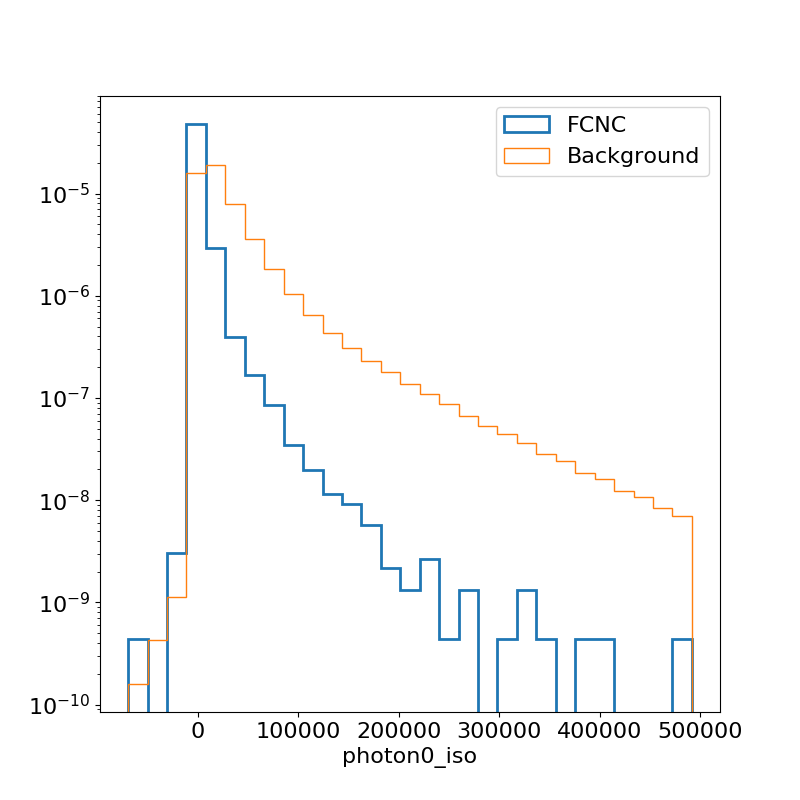
\includegraphics[width=.4\columnwidth]{../ThesisImages/SearchStrategy/varplots/photon0_iso.png}}\hfil
\subfloat[$\gamma_{p_T}$]{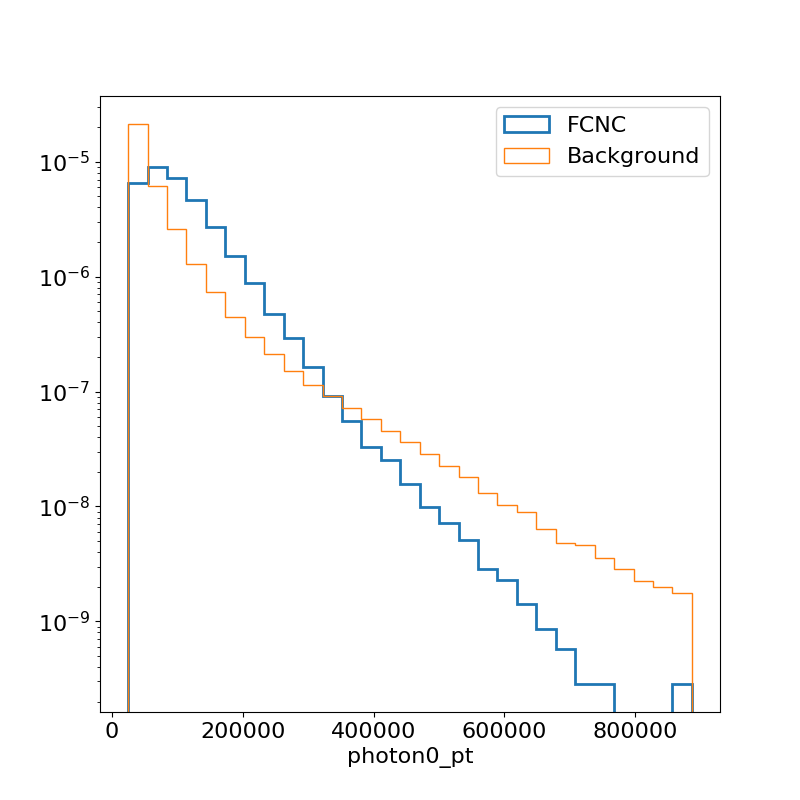
\includegraphics[width=.4\columnwidth]{../ThesisImages/SearchStrategy/varplots/photon0_pt.png}}
\vspace{-4.5mm}
\subfloat[$m_{q \gamma}$]{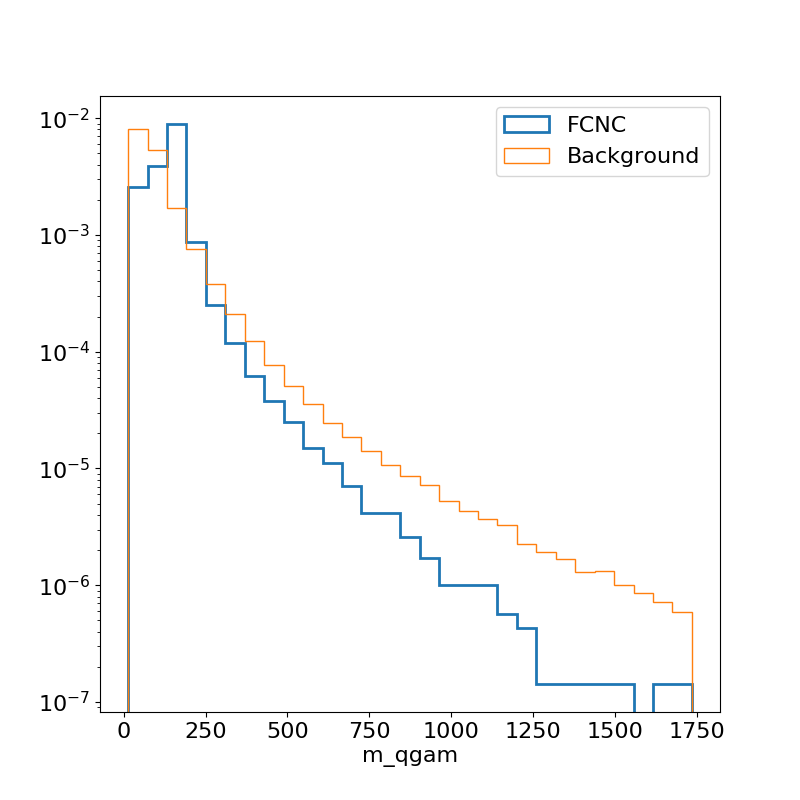
\includegraphics[width=.4\columnwidth]{../ThesisImages/SearchStrategy/varplots/m_qgam.png}}\hfil
\subfloat[$m_{l \gamma}$]{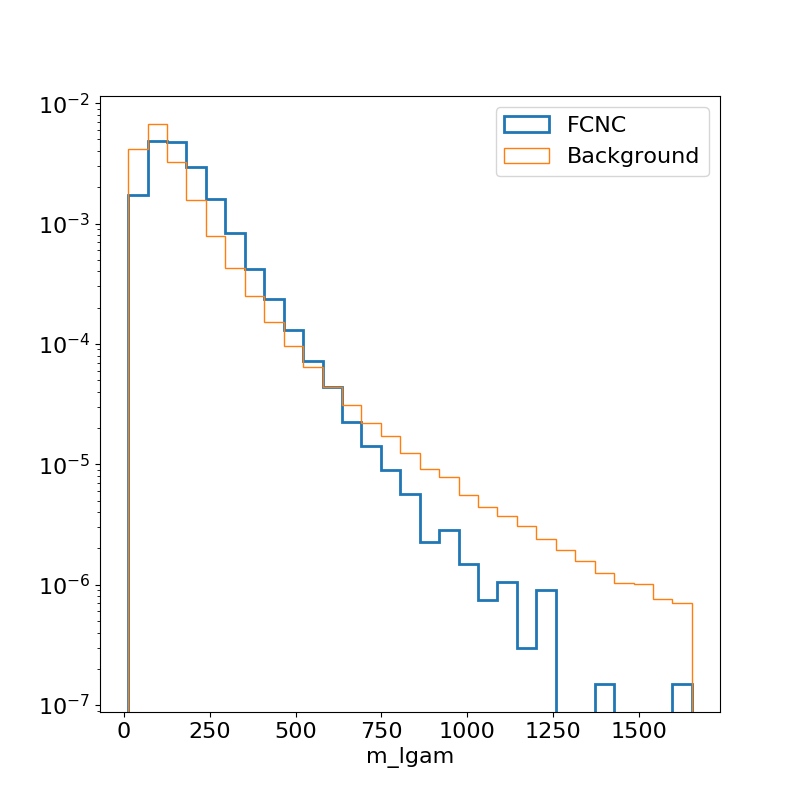
\includegraphics[width=.4\columnwidth]{../ThesisImages/SearchStrategy/varplots/m_lgam.png}}   
\vspace{-4.5mm}
\subfloat[$m_{bW}$]{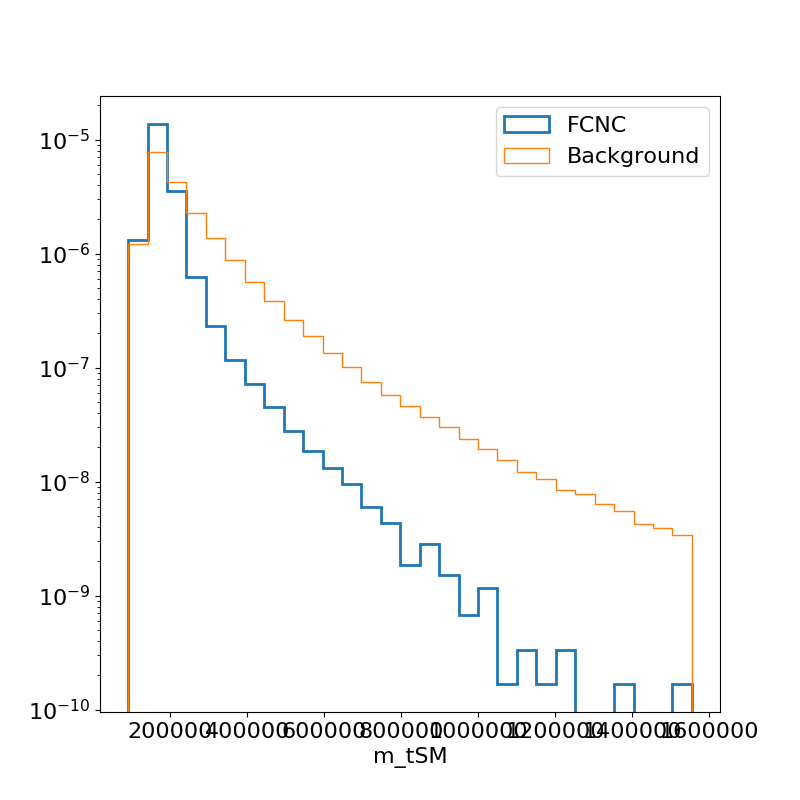
\includegraphics[width=.4\columnwidth]{../ThesisImages/SearchStrategy/varplots/m_tSM.png}}\hfil
\subfloat[$\Delta R_{j\gamma}$]{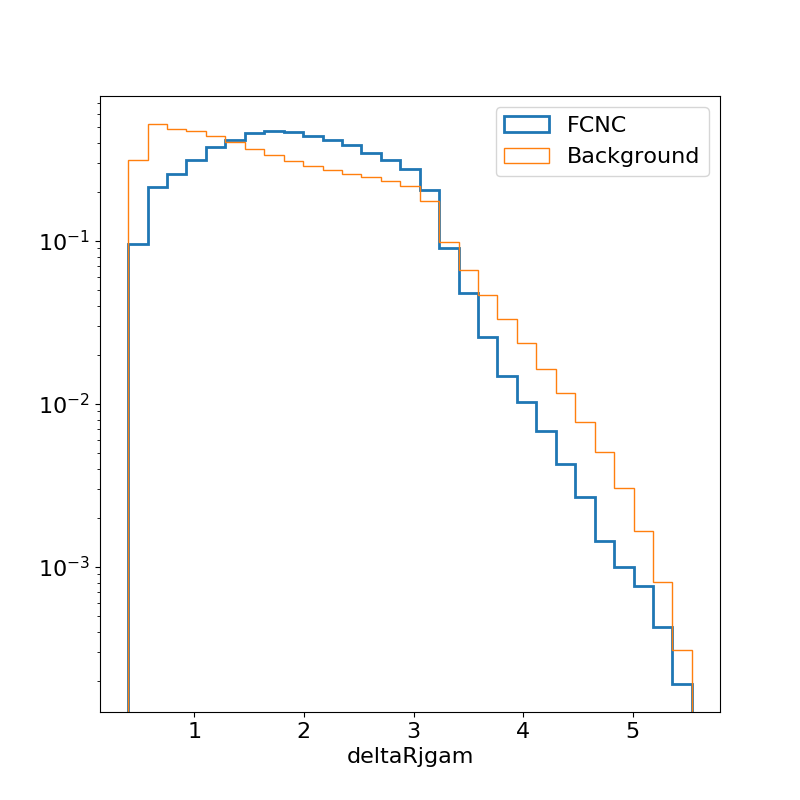
\includegraphics[width=.4\columnwidth]{../ThesisImages/SearchStrategy/varplots/deltaRjgam.png}}
\caption{Normalized variables showing the shapes of neural network input variables for the $\mu$+jets channel: $\gamma_{iso}$ topo$E_{T}$cone40, $\gamma_{p_T}$, $m_{q \gamma}$, $m_{l \gamma}$, $m_{bW}$, and $\Delta R_{j\gamma}$ }
\label{fig:VarPlots1}
\end{figure}



\begin{figure}[h!]
\centering
\subfloat[$\Delta R_{b l}$]{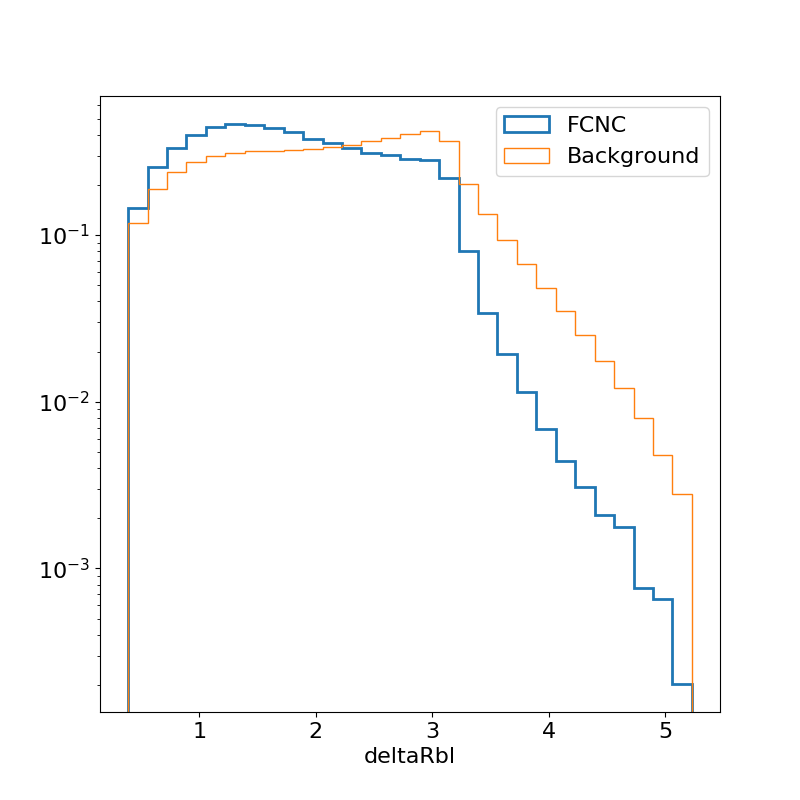
\includegraphics[width=.4\columnwidth]{../ThesisImages/SearchStrategy/varplots/deltaRbl.png}}\hfil
\subfloat[$m_{T}^{W}$ ]{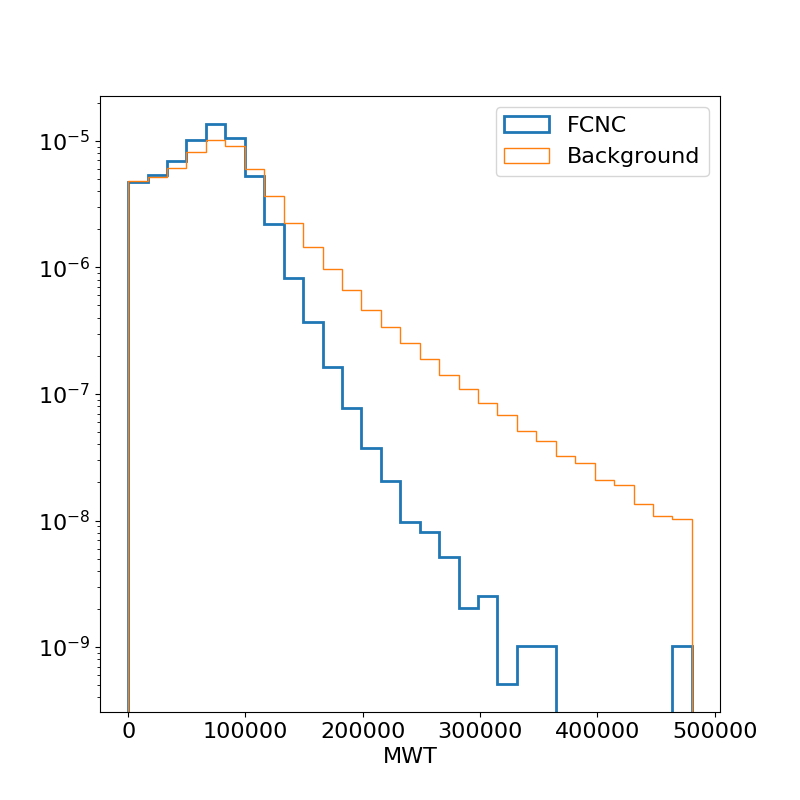
\includegraphics[width=.4\columnwidth]{../ThesisImages/SearchStrategy/varplots/MWT.png}}
\vspace{-4.5mm}
\subfloat[$S_T$]{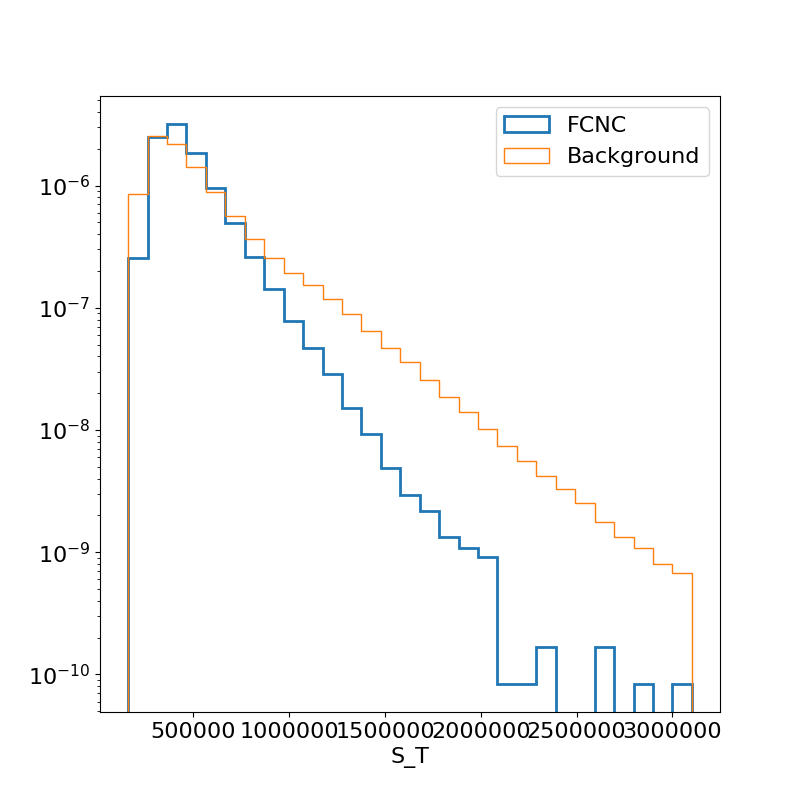
\includegraphics[width=.4\columnwidth]{../ThesisImages/SearchStrategy/varplots/S_T.png}}\hfil
\subfloat[$n_{\text{jets}}$]{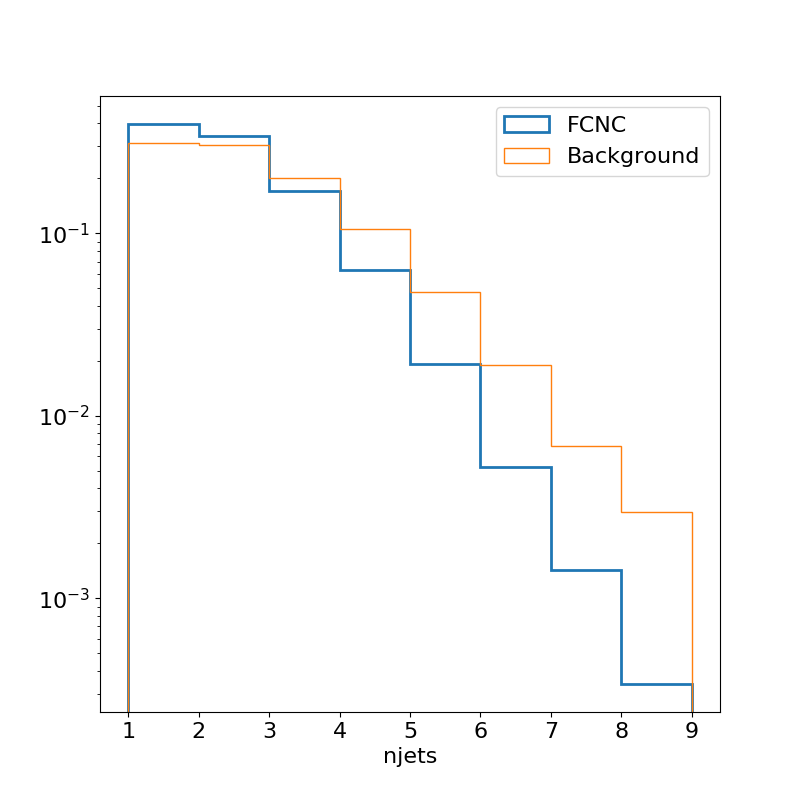
\includegraphics[width=.4\columnwidth]{../ThesisImages/SearchStrategy/varplots/njets.png}}   
\vspace{-4.5mm}
\subfloat[$\chi^{2}_{W}$]{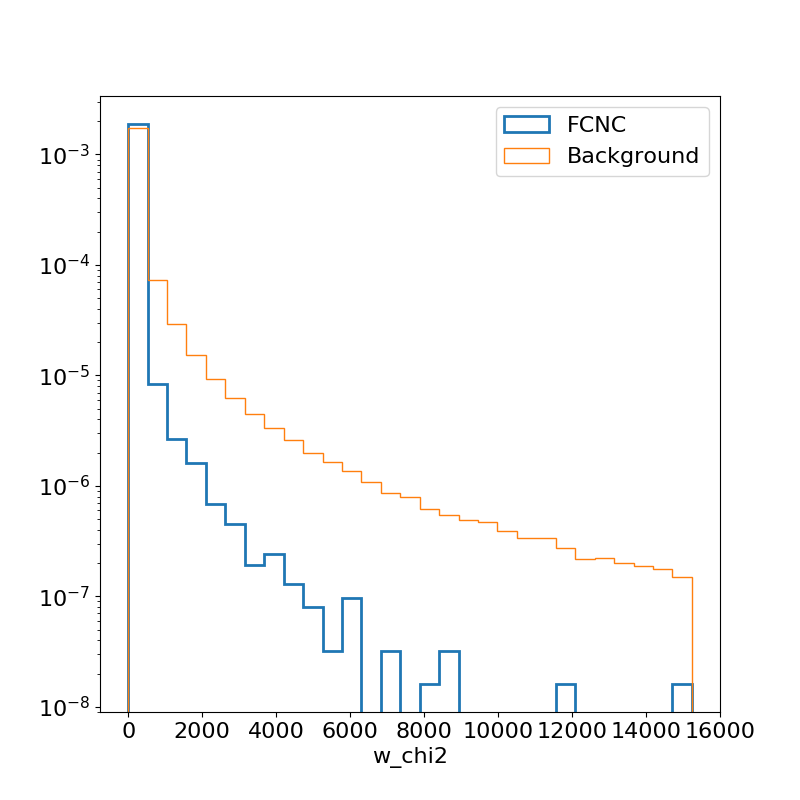
\includegraphics[width=.4\columnwidth]{../ThesisImages/SearchStrategy/varplots/w_chi2.png}}\hfil
\subfloat[$p_T (q)$]{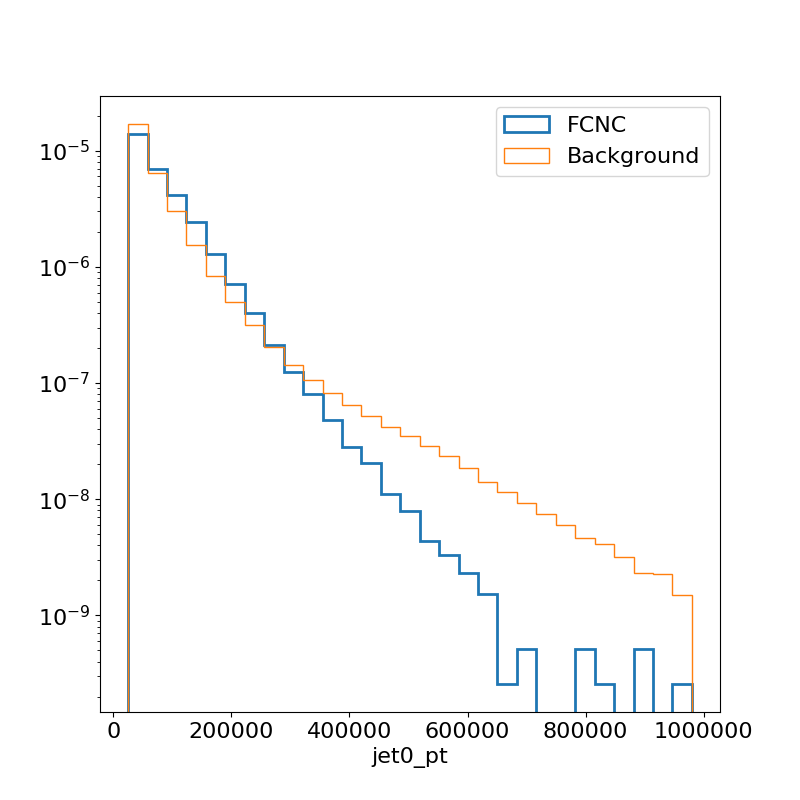
\includegraphics[width=.4\columnwidth]{../ThesisImages/SearchStrategy/varplots/jet0_pt.png}}
\caption{Normalized variables showing the shapes of neural network input variables for the $\mu$+jets channel: $\Delta R_{b l}$, $m_{T}^{W}$ , $S_T$, $n_{\text{jets}}$, $\chi^{2}_{W}$, and $p_T (q)$}
\label{fig:VarPlots2}
\end{figure}

\begin{figure}[h!]
\centering
\subfloat[$\Delta R_{l \gamma}$]{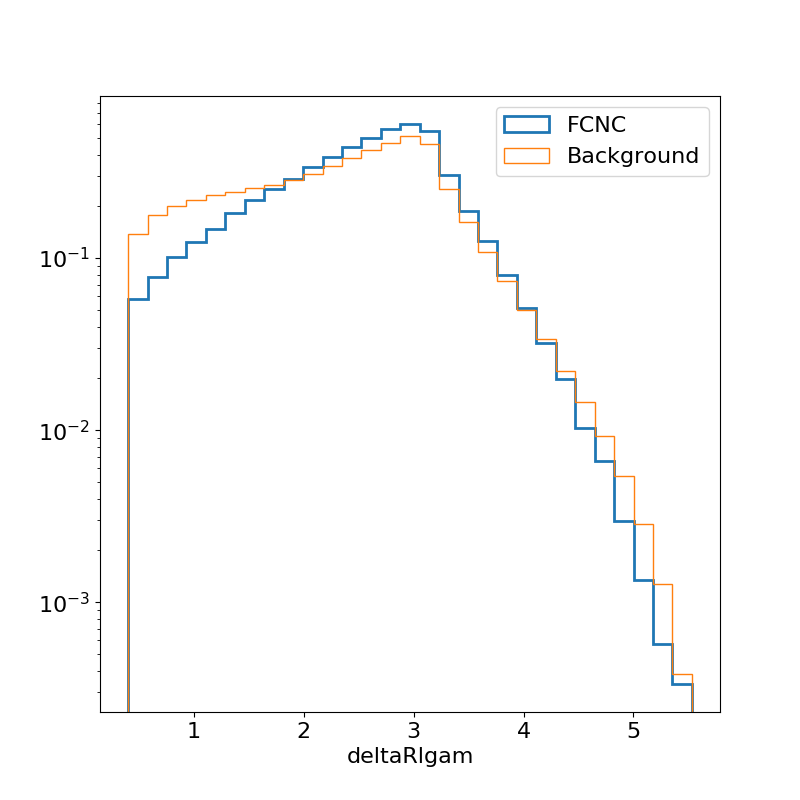
\includegraphics[width=.4\columnwidth]{../ThesisImages/SearchStrategy/varplots/deltaRlgam.png}}\hfil
\subfloat[E (lepton)]{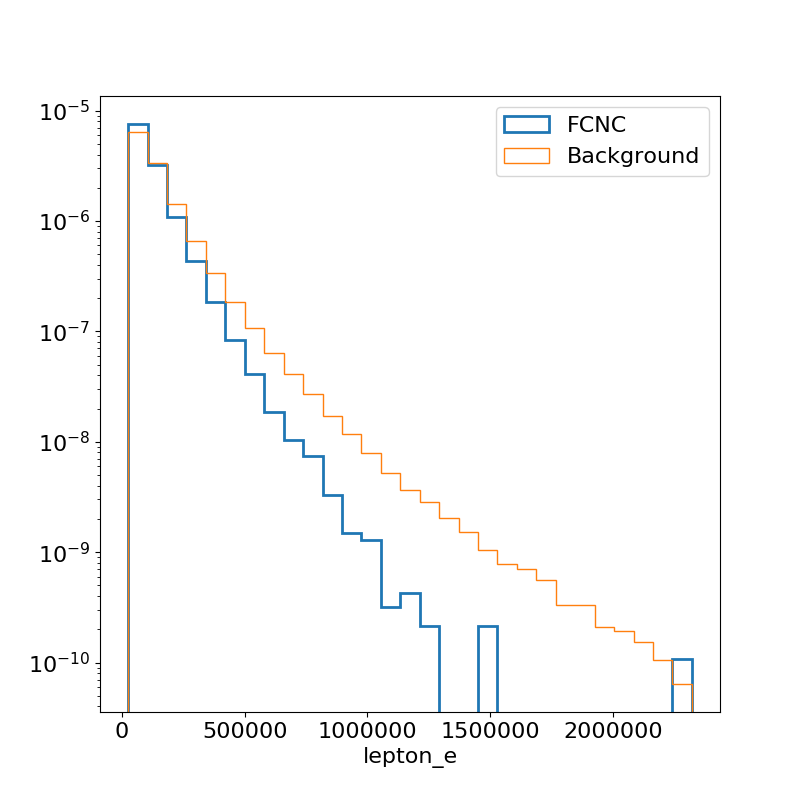
\includegraphics[width=.4\columnwidth]{../ThesisImages/SearchStrategy/varplots/lepton_e.png}}
\vspace{-4.5mm}
\subfloat[$\slashed{E}_T  $]{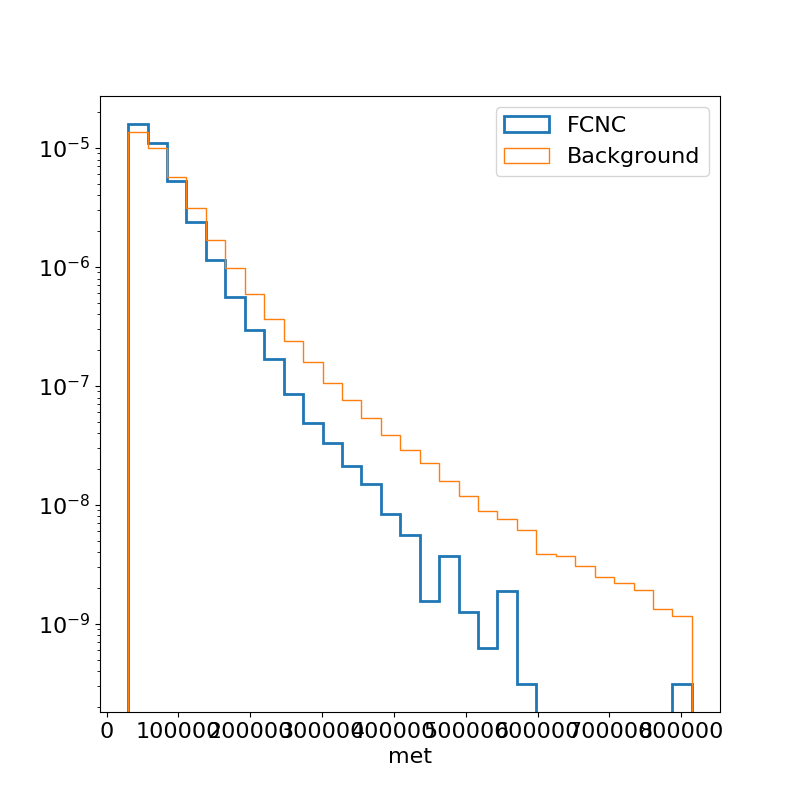
\includegraphics[width=.4\columnwidth]{../ThesisImages/SearchStrategy/varplots/met.png}}\hfil
\subfloat[$p_T (b)$ ]{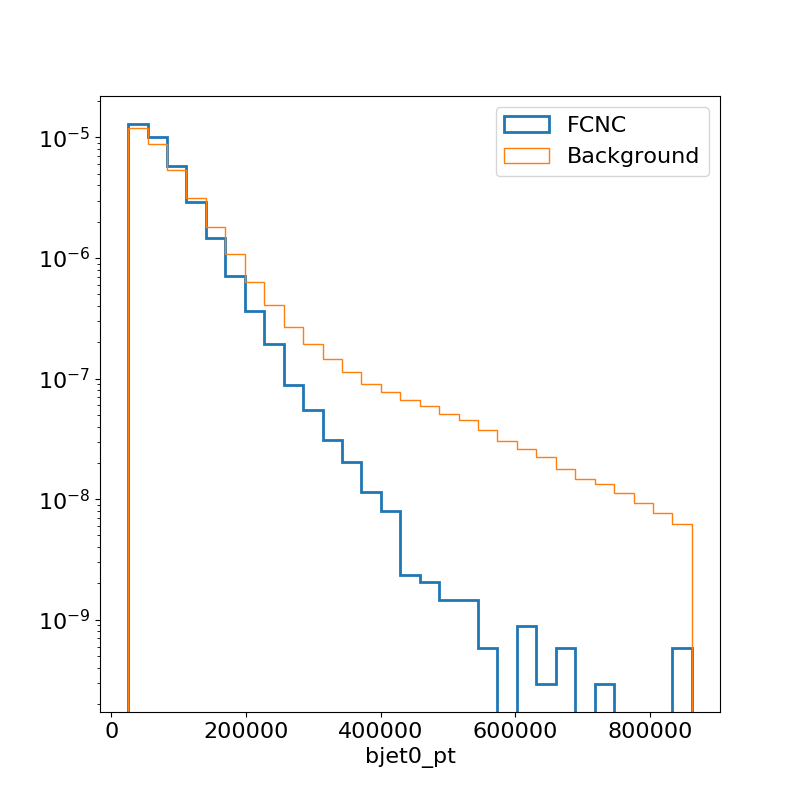
\includegraphics[width=.4\columnwidth]{../ThesisImages/SearchStrategy/varplots/bjet0_pt.png}}   
\caption{Normalized variables showing the shapes of neural network input variables for the $\mu$+jets channel: $\Delta R_{l \gamma}$, E (lepton), $\slashed{E}_T  $, and $p_T (b)$}
\label{fig:VarPlots3}
\end{figure}


\subsection{Architecture}

A variety of architectures of dense neural networks are studied using \textsc{Keras}\cite{Keras} on top of the \textsc{TensorFlow} backend \cite{TensorFlow}.  Each network has a number of input nodes equal to the number of input variables.  Networks with one, two, and three hidden layers are investigated each with 20 nodes.  The output layer contains only a single node.  Every node in one layer is connected to every node in the next layer and the previous layer.  Every connection is assigned a weight that is optimized during the training of the network.  For every node in the network a value is computed using the weights and input values of the previous nodes using an activation function.  Nodes with the highest output of this function are more important to the fit.  The activation function used on the internal nodes in this search is the Rectified Linear Unit activation function.
\[ ReLU(x) = 
\begin{cases}
x, \qquad \text{if } x \geq 0\\
0, \qquad \text{if } x < 0
\end{cases}
\]
The output layer uses the sigmoid function, $\sigma(x)$, as an activation function.  The sigmoid function maps the output smoothly to the range (0,1).
\[ \sigma(x) = \frac{1}{1+e^{-x}}
\]
In every training step the weights of each node are updated following an optimization algorithm, in this case the \textsc{Adam} optimizer\cite{AdamOpt}.  This optimizer follows the steepest gradient to reach the minimum of the parameter of interest called the loss function.  The loss function used for these classification neural networks is the binary cross entropy:
\[\text{Loss} = -\frac{1}{N}\sum_{i=1}^{N}y_{i} \text{log}(p(y_{i}))+(1-y_{i})\text{log}(1-p(y_{i}))\]
where $y$ is a binary indicator (0 or 1) if class label is the correct classification for observation and $p$ is the predicted probability observation of the class label (0 or 1).  The logarithmic nature of this loss function means it applys small values to correctly assigned events but more harshly punishes mismatching of events.  Therefore having a similar number of signal and background events that get weighted similarly can improve the behavior of the network.  In rare decay searches typically the amount of signal events is significantly smaller than the amount of background events in the training sample.  By using the weight functionality in \textsc{Keras}, the total number of signal events can be scaled to be similar to the number of background events. 

Weighting the signal events this way allows the network to separate the signal and background events in a way that is significantly less harsh than without the weights by taking advantage of the loss function being used.  This improves the estimated significance of the neural network cut after the signal events are rescaled to their proper normalization values.  

\begin{figure}[h!]
	\centering
	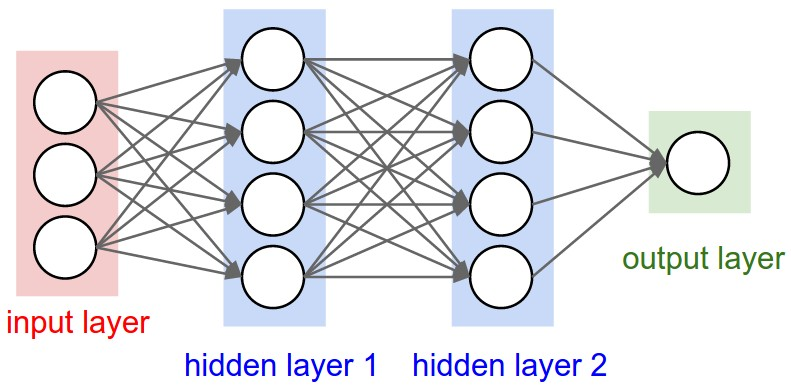
\includegraphics[width=\columnwidth]{../ThesisImages/SearchStrategy/neural_net2.jpeg}
	\caption[Pictoral representation of neural network architecture with 3 input variables, 2 hidden layers with 4 nodes each, and 1 output layer.]{Pictoral representation of neural network architecture with 3 input variables, 2 hidden layers with 4 nodes each, and 1 output layer\cite{NNImage}.}
	\label{fig:NNArch}
\end{figure}

Various hyperparameters are used as inputs into the neural network as well as the optimizer used.  The \textsc{Adam} optimizer has a default learning rate of 0.001 which remained constant throughout these studies.   The learning rate corresponds to the amount that weights are updated during training.  A learning rate that is too large can mean the network never settles into a local minima as it is always missing the minima or, at the very least, it can take much longer to converge into a minima.  As the neural network training for this search always converged quickly and to a similar value after being tested multiple different times the learning rate was not adapted.  

Another hyperparameter of note is the batch size that defines the number of samples that are propagated through the network at once.  The batch size is crucial in determining how long the training of the network takes.  A set of 1000 training samples with a batch size of 100 will propagate each set of 100 samples through the neural network every epoch, so 10 separate batches.  A larger batch size means that each epoch of the training takes a shorter amount of time.  However, as the weights are updated after each batch the network can take many more epochs to converge as the weights are being updated less frequently.  A batch size of 100 was used while training the networks presented in this chapter.  Larger batch sizes were tested with the only difference being the time each epoch took and the total time the network took to converge.

Epochs are the total number of times the network has been trained over the entire training set.  All of the networks were allowed up to 200 epochs to converge with a \textsc{Keras} patience value set to 50.  The loss function minimization would be done every batch and after each epoch the best possible value of the loss function is found.  If this value is better than any previous epoch the network is allowed to train for 50 more epochs until 50 epochs have passed without finding a new minimum loss function value which then terminates the training.  All models converge early and are terminated typically between epoch 80 and 120 meaning the loss function was minimized between epoch 30 and 70.  

One method employed to avoid overtraining the network dropout regularization was used on each of the hidden layers.  Dropout has the effect of simulating a large number of networks with very different network structures by removing nodes randomly throughout the training. A dropout rate of 20\% was used, meaning that for every batch 20\% of the weights of the hidden layer nodes were set to 0.  This prevents the network from becoming overly dependent on any given node or learning the data `by heart' as opposed to recognizing the trends in the sample. 

\subsubsection{Training and Validation of Neural Networks}

The input variables into the neural network are preprocessed using the \textsc{RobustScalar} method implemented in \textbf{scikit-learn}\cite{ScikitLearn}.  The preprocessing is done so that the input variables exist on a similar scale.  As the network is tasked with learning how to combine these inputs through a series of linear combinations and nonlinear activation function values, a disparity in the scales of the input values can lead to awkward loss function topology that focuses on certain parameter gradients instead of treating them all similarly.  Normalizing the values to a standard scale allows the network to learn the optimal parameters for each input node more quickly and efficiently.  This means that less focus can be used on the optimization of the hyperparameters for the network as the scales of the inputs do not need to be learned by the network itself.

Each input variable in the neural network, $x$, is scaled by the following equation:
\[ z = \frac{x - m }{q_3 - q_1} \]
where $m$ is the median of the distribution, and $q_1$ and $q_3$ are the first and third quartile.  This changes the distribution of the input variable distributions to be centered around zero.

A second method to avoid overtraining the neural network is to make use of a train-test split to split the signal and background samples into 3 independent randomized sets before training the neural network.  The samples are split into a training set of 64\% of the samples, a test set  containing 20\% of the samples, and the remaing 16\% are a validation set.  The training and test sets are used during the training of the network while the validation set is used to compute performance of the trained neural network.

One measure of the performance of the network is the accuracy. The \textsc{Keras} default accuracy measure is defined:
\[ \text{accuracy} = \frac{N(\text{event}_{NN} \geq 0.5|\text{signal})+ N(\text{event}_{NN} <0.5|\text{background})}{N(\text{signal})+N(\text{background})} \]
where $N(\text{event}_{NN} \geq 0.5|\text{signal})$ ($N(\text{event}_{NN} \geq 0.5|\text{signal})$) is the number of signal (background) events with $P_{\text{signal}}\geq 0.5$ ($P_{\text{signal}}< 0.5$).  Essentially, the accuracy is a measure of the mean of how often correct prediction values occur assuming a cut on the output of $\geq0.5$.

% EJets Train Test Split
% train, test, val
% Sig: (72589, 47) (22685, 47) (18148, 47)
%ttbar (963721, 47) (301163, 47) (240931, 47)
%singleTop (56456, 47) (17643, 47) (14114, 47)
%ttV (190610, 47) (59566, 47) (47653, 47)
%diboson (68024, 47) (21258, 47) (17007, 47)
%WJets (195049, 47) (60953, 47) (48763, 47)
%ZJets (314462, 47) (98270, 47) (78616, 47)
%Mujets train Test Val
%Sig: (75607, 47) (23628, 47) (18902, 47)
%ttbar (912851, 47) (285266, 47) (228213, 47)
%singleTop (53772, 47) (16804, 47) (13444, 47)
%ttV (153174, 47) (47868, 47) (38294, 47)
%diboson (45536, 47) (14231, 47) (11384, 47)
%WJets (189872, 47) (59335, 47) (47468, 47)
%ZJets (104734, 47) (32730, 47) (26184, 47)
% 80% train, 20% test
% 80% newtrain, 20% val

%%%%%%%%%% Show outputs for a network, give examples all my pretty plots

\subsection{Hidden Layer Studies}
\label{sec:HiddenStudies}
The general performance of the neural network was studied with a varying number of hidden layers (1, 2, and 3) in both the $e$+jets and $\mu$+jets channels.   All of the networks are trained on the same set of variables and with the same train-test split input data.  For each of the channels the \textit{Receiver Operating Characterisitic} (ROC) curves are shown in Figure \ref{fig:ROCHidden}.  The ROC curves show the value of $1-\epsilon_{\text{bkg}}$ as a function of the true positive rate, $\epsilon_{\text{signal}}$.  A figure of merit is the Area Under the Curve (AUC) which is a measure of how close the resulting values are to the optimal value of unity. 

\begin{figure}[h!]
\centering
\subfloat[$e$+jets ROC Curves]{\includegraphics[width=.5\columnwidth]{../ThesisImages/SearchStrategy/{HiddenLayerStudiesBR0.002}/btag77/modelouts/ejetsbothroc.png}}\hfil
\subfloat[$\mu$+jets ROC Curves]{\includegraphics[width=.5\columnwidth]{../ThesisImages/SearchStrategy/{HiddenLayerStudiesBR0.002}/btag77/modelouts/mujetsbothroc.png}}
\caption{ROC Curves are shown for both search channels for a varying number of hidden layers. Orange lines correspond to one hidden layer, blue to 2 hidden layers and green to 3 hidden layers.  The blue and green curves have near identical AUC values: 0.950 and 0.951 for the $e$+jets case and $0.962$ for the $\mu$+jets cases.}
\label{fig:ROCHidden}
\end{figure}

The AUC for 2 hidden layers and 3 hidden layers are identical within rounding errors for both channels.  As such the network with 2 hidden layers has been chosen as it is computationally simpler.   The normalized neural network output values are shown in Figure \ref{fig:HiddenSigBkg}.  Adding a second hidden layer significantly improves the performance of the network but a third layer does not.  The output shapes change slightly when the third hidden layer is added due to the network learning differently from similar data.  However, as the AUC shows, the performance of 2 and 3 hidden layers is identical.   Figures \ref{fig:Acc2Hid} and \ref{fig:Loss2Hid} show the accuracy metric and the loss function as a function of the training epoch for the networks trained with 2 hidden layers.   The accuracy plot behavior is expected as the validation data sets do not have dropout regularization applied to them.  These networks are also trained without further reduction of Z+jets background meaning the $e$+jets sample has a larger background contamination that makes the validation testing more volatile.  This is due to the increased number of similar events in that sample that can be more heavily dependent on specific weights across the network for identification.

\begin{figure}[h!]
\centering
\subfloat[$e$+jets Accuracy Curves]{\includegraphics[width=.5\columnwidth]{../ThesisImages/SearchStrategy/{HiddenLayerStudiesBR0.002}/BestResults/btag77/ejetsboth2hidnpart0accuarcy.png}}\hfil
\subfloat[$\mu$+jets Accuracy Curves]{\includegraphics[width=.5\columnwidth]{../ThesisImages/SearchStrategy/{HiddenLayerStudiesBR0.002}/BestResults/btag77/mujetsboth2hidnpart0accuarcy.png}}
\caption{Accuracy plots for both channels for the 2 hidden layer neural network}
\label{fig:Acc2Hid}
\end{figure}

\begin{figure}[h!]
\centering
\subfloat[$e$+jets Loss Curve]{\includegraphics[width=.5\columnwidth]{../ThesisImages/SearchStrategy/{HiddenLayerStudiesBR0.002}/BestResults/btag77/ejetsboth2hidnpart0loss.png}}\hfil
\subfloat[$\mu$+jets Loss Curve]{\includegraphics[width=.5\columnwidth]{../ThesisImages/SearchStrategy/{HiddenLayerStudiesBR0.002}/BestResults/btag77/mujetsboth2hidnpart0loss.png}}
\caption{Loss plots for both channels for the 2 hidden layer neural network}
\label{fig:Loss2Hid}
\end{figure}

The main metric used in choosing which network has the best physics reach is the significance:
\[ \text{significance} = \frac{N_{s}}{\sqrt{N_s +N_b}}\]
where $N_{s}$ is the number of signal events that pass the cut and $N_b$ is the number of background events that pass the neural network cut.
After the model has been fully trained, it is tested on all of the Monte Carlo for signal and background.  The signal samples are normalized to various branching ratios (in the range $10^{-5}\rightarrow 3\times 10^{-3}$) and full LHC Run-2 luminosity, and the significance is calculated as a function of the cut on the output of the neural network $P(\text{signal})$.  The network with the output cut for the smallest branching ratio with a maximum significance of 2 is chosen, a rough estimate of where the expected limit could be set.  The significance as a function of the neural network output cut is shown in Figure \ref{fig:Sig2Hid}.
\begin{figure}[h!]
\centering
\subfloat[$e$+jets:1 Hidden Layer]{\includegraphics[width=.33\columnwidth]{../ThesisImages/SearchStrategy/{HiddenLayerStudiesBR0.002}/btag77/modelouts/ejetsboth1hidnpart0sigbkg.png}}\hfil
\subfloat[$e$+jets:2 Hidden Layers]{\includegraphics[width=.33\columnwidth]{../ThesisImages/SearchStrategy/{HiddenLayerStudiesBR0.002}/btag77/modelouts/ejetsboth2hidnpart0sigbkg.png}}\hfil
\subfloat[$e$+jets:3 Hidden Layers]{\includegraphics[width=.33\columnwidth]{../ThesisImages/SearchStrategy/{HiddenLayerStudiesBR0.002}/btag77/modelouts/ejetsboth3hidnpart0sigbkg.png}}
\vspace{-3.mm}
\subfloat[$\mu$+jets:1 Hidden Layer]{\includegraphics[width=.33\columnwidth]{../ThesisImages/SearchStrategy/{HiddenLayerStudiesBR0.002}/btag77/modelouts/mujetsboth1hidnpart0sigbkg.png}}\hfil
\subfloat[$\mu$+jets:2 Hidden Layers]{\includegraphics[width=.33\columnwidth]{../ThesisImages/SearchStrategy/{HiddenLayerStudiesBR0.002}/btag77/modelouts/mujetsboth2hidnpart0sigbkg.png}}\hfil
\subfloat[$\mu$+jets:3 Hidden Layers]{\includegraphics[width=.33\columnwidth]{../ThesisImages/SearchStrategy/{HiddenLayerStudiesBR0.002}/btag77/modelouts/mujetsboth3hidnpart0sigbkg.png}}
\caption{Normalized neural network output signal and background distribution plots are shown for both search channels for a varying number of hidden layers.}
\label{fig:HiddenSigBkg}
\end{figure}

\begin{figure}[h!]
\centering
\subfloat[$e$+jets]{\includegraphics[width=.5\columnwidth]{../ThesisImages/SearchStrategy/{HiddenLayerStudiesBR0.002}/BestResults/btag77/significanceejetsboth2hidnpart02.png}}\hfil
\subfloat[$\mu$+jets]{\includegraphics[width=.5\columnwidth]{../ThesisImages/SearchStrategy/{HiddenLayerStudiesBR0.002}/BestResults/btag77/significancemujetsboth2hidnpart02.png}}
\caption[Significance plots for both channels for the 2 hidden layer neural network.]{Significance plots for both channels for the 2 hidden layer neural network.  The green points correspond to a branching ratio with a maximum significance of 5, and the orange to a maximum significance of 2.  The $e$+jets ($\mu$+jets) branching ratio with max significance of 2 is $1.22 \times10^{-5} (1.18\times10^{-5})$. The blue, red, purple, and brown points correspond to branching ratios of  $1\times10^{-5}$, $5\times10^{-4}$, $1\times10^{-3}$, and $5\times10^{-3}$, respectively.}
\label{fig:Sig2Hid}
\end{figure}


\subsection{B-Tagging Working Point Studies}
\label{sec:btagNN}
The b-tagging working point selection was performed with similar neural network studies.  Three neural networks were trained with the datasets using the jet information and total scaled events for each of the major b-tagging working points: 70\%, 77\%, and 85\%.  Changing the working point alters a number of things about the signal and background data sets such as which jets are b tagged and therefore which jets are combined into the higher level variables (e.g., $m_{q\gamma}$ and $m_{Wb}$).  The total number of events that pass the pre-selection to the neural network is also changed for all of the datasets since the neural networks are only trained on events with 1 b-tagged jet.  Similar sets of plots to Section \ref{sec:HiddenStudies} will be presented in this section.

This selection of neural networks were trained in parallel with one, two, and three hidden layers.  The only results shown are the 2 hidden layer outputs as they perform equally or better than the others as previously discussed.  The accuracy and loss plots for these networks are shown in Figures \ref{fig:BTagEAccLoss} and \ref{fig:BTagMuAccLoss}.  The neural network output and significance plots shown in Figures \ref{fig:BTagEOutSig} and \ref{fig:BTagMuOutSig} follow.  

\begin{figure}[h!]
\centering
\subfloat[70\% WP Loss]{\includegraphics[width=.33\columnwidth]{../ThesisImages/SearchStrategy/{HiddenLayerStudiesBR0.002}/BestResults/btag70/ejetsboth2hidnpart0loss.png}}\hfil
\subfloat[77\% WP Loss]{\includegraphics[width=.33\columnwidth]{../ThesisImages/SearchStrategy/{HiddenLayerStudiesBR0.002}/BestResults/btag77/ejetsboth2hidnpart0loss.png}}\hfil
\subfloat[85\% WP Loss]{\includegraphics[width=.33\columnwidth]{../ThesisImages/SearchStrategy/{HiddenLayerStudiesBR0.002}/BestResults/btag85/ejetsboth2hidnpart0loss.png}}
\vspace{-3.mm}
\subfloat[70\% WP Accuracy]{\includegraphics[width=.33\columnwidth]{../ThesisImages/SearchStrategy/{HiddenLayerStudiesBR0.002}/BestResults/btag70/ejetsboth2hidnpart0accuarcy.png}}\hfil
\subfloat[77\% WP Accuracy]{\includegraphics[width=.33\columnwidth]{../ThesisImages/SearchStrategy/{HiddenLayerStudiesBR0.002}/BestResults/btag77/ejetsboth2hidnpart0accuarcy.png}}\hfil
\subfloat[85\% WP Accuracy]{\includegraphics[width=.33\columnwidth]{../ThesisImages/SearchStrategy/{HiddenLayerStudiesBR0.002}/BestResults/btag85/ejetsboth2hidnpart0accuarcy.png}}
\caption{Accuracy and loss plots for the $e$+jets channel at 70\%, 77\%, and 85\% b-tagging working points.}
\label{fig:BTagEAccLoss}
\end{figure}

\begin{figure}[h!]
\centering
\subfloat[70\% WP Loss]{\includegraphics[width=.33\columnwidth]{../ThesisImages/SearchStrategy/{HiddenLayerStudiesBR0.002}/BestResults/btag70/mujetsboth2hidnpart0loss.png}}\hfil
\subfloat[77\% WP Loss]{\includegraphics[width=.33\columnwidth]{../ThesisImages/SearchStrategy/{HiddenLayerStudiesBR0.002}/BestResults/btag77/mujetsboth2hidnpart0loss.png}}\hfil
\subfloat[85\% WP Loss]{\includegraphics[width=.33\columnwidth]{../ThesisImages/SearchStrategy/{HiddenLayerStudiesBR0.002}/BestResults/btag85/mujetsboth2hidnpart0loss.png}}
\vspace{-3.mm}
\subfloat[70\% WP Accuracy]{\includegraphics[width=.33\columnwidth]{../ThesisImages/SearchStrategy/{HiddenLayerStudiesBR0.002}/BestResults/btag70/mujetsboth2hidnpart0accuarcy.png}}\hfil
\subfloat[77\% WP Accuracy]{\includegraphics[width=.33\columnwidth]{../ThesisImages/SearchStrategy/{HiddenLayerStudiesBR0.002}/BestResults/btag77/mujetsboth2hidnpart0accuarcy.png}}\hfil
\subfloat[85\% WP Accuracy]{\includegraphics[width=.33\columnwidth]{../ThesisImages/SearchStrategy/{HiddenLayerStudiesBR0.002}/BestResults/btag85/mujetsboth2hidnpart0accuarcy.png}}
\caption{Accuracy and loss plots for the $\mu$+jets channel at 70\%, 77\%, and 85\% b-tagging working points.}
\label{fig:BTagMuAccLoss}
\end{figure}

\begin{figure}[h!]
\centering
\subfloat[70\% WP NN output]{\includegraphics[width=.33\columnwidth]{../ThesisImages/SearchStrategy/{HiddenLayerStudiesBR0.002}/BestResults/btag70/ejetsboth2hidnpart0sigbkg.png}}\hfil
\subfloat[77\% WP NN output]{\includegraphics[width=.33\columnwidth]{../ThesisImages/SearchStrategy/{HiddenLayerStudiesBR0.002}/BestResults/btag77/ejetsboth2hidnpart0sigbkg.png}}\hfil
\subfloat[85\% WP NN output]{\includegraphics[width=.33\columnwidth]{../ThesisImages/SearchStrategy/{HiddenLayerStudiesBR0.002}/BestResults/btag85/ejetsboth2hidnpart0sigbkg.png}}
\vspace{-3.mm}
\subfloat[70\% WP Significance]{\includegraphics[width=.33\columnwidth]{../ThesisImages/SearchStrategy/{HiddenLayerStudiesBR0.002}/BestResults/btag70/significanceejetsboth2hidnpart02.png}}\hfil
\subfloat[77\% WP Significance]{\includegraphics[width=.33\columnwidth]{../ThesisImages/SearchStrategy/{HiddenLayerStudiesBR0.002}/BestResults/btag77/significanceejetsboth2hidnpart02.png}}\hfil
\subfloat[85\% WP Significance]{\includegraphics[width=.33\columnwidth]{../ThesisImages/SearchStrategy/{HiddenLayerStudiesBR0.002}/BestResults/btag85/significanceejetsboth2hidnpart02.png}}
\caption{Neural network output and significance plots for the $e$+jets channel at 70\%, 77\%, and 85\% b-tagging working points.}
\label{fig:BTagEOutSig}
\end{figure}

\begin{figure}[h!]
\centering
\subfloat[70\% WP NN output]{\includegraphics[width=.33\columnwidth]{../ThesisImages/SearchStrategy/{HiddenLayerStudiesBR0.002}/BestResults/btag70/mujetsboth2hidnpart0sigbkg.png}}\hfil
\subfloat[77\% WP NN output]{\includegraphics[width=.33\columnwidth]{../ThesisImages/SearchStrategy/{HiddenLayerStudiesBR0.002}/BestResults/btag77/mujetsboth2hidnpart0sigbkg.png}}\hfil
\subfloat[85\% WP NN output]{\includegraphics[width=.33\columnwidth]{../ThesisImages/SearchStrategy/{HiddenLayerStudiesBR0.002}/BestResults/btag85/mujetsboth2hidnpart0sigbkg.png}}
\vspace{-3.mm}
\subfloat[70\% WP Significance]{\includegraphics[width=.33\columnwidth]{../ThesisImages/SearchStrategy/{HiddenLayerStudiesBR0.002}/BestResults/btag70/significancemujetsboth2hidnpart02.png}}\hfil
\subfloat[77\% WP Significance]{\includegraphics[width=.33\columnwidth]{../ThesisImages/SearchStrategy/{HiddenLayerStudiesBR0.002}/BestResults/btag77/significancemujetsboth2hidnpart02.png}}\hfil
\subfloat[85\% WP Significance]{\includegraphics[width=.33\columnwidth]{../ThesisImages/SearchStrategy/{HiddenLayerStudiesBR0.002}/BestResults/btag85/significancemujetsboth2hidnpart02.png}}
\caption{Neural network output and significance plots for the $\mu$+jets channel at 70\%, 77\%, and 85\% b-tagging working points.}
\label{fig:BTagMuOutSig}
\end{figure}

The result of these studies is the choice of using the 77\% working point for b-tagged jets.  The branching ratio with significance of 2 is found for each network and reported in Table \ref{tab:BRsAfterNN}.

\begin{table}[]
\begin{center}
{\renewcommand{\arraystretch}{1.2}
\begin{tabular}{ccc}
\hline
B-Tag Working Point  &  $e$+jets Branching Ratio   & $\mu$+jets Branching Ratio  \\  \hline 
70\%            &  $1.25\times10^{-5}$  &  $1.31\times10^{-5}$\\
77\%           &   $1.23\times10^{-5}$ &   $1.18\times10^{-5}$	\\  
85\%            &  $1.27\times10^{-5}$ &   $1.19\times10^{-5}$	\\ \hline
\end{tabular}
\caption{Branching ratio values with a significance of 2 after neural network optimization}
\label{tab:BRsAfterNN}
}
\end{center}
\end{table}


%\subsection{Comparison of FCNC in Decay and Production via the Neural Network}

%%%%%%%%%%%%%%%%%%%%%%%%%%%%%%%%%%%%%%%%%%%%%%
%%%%%%%%%  									        	 %%%%%%%%
%%%%%%%%%                     End of Neural Net Section                                             %%%%%%%%
%%%%%%%%%										 %%%%%%%%
%%%%%%%%%%%%%%%%%%%%%%%%%%%%%%%%%%%%%%%%%%%%%%


\section{Initial Event Selection}
\label{sec:InitSelec}
Initial event selection is done to ensure that the events accepted into the analysis are not contaminated by extremely noisy detector environments and that these events happened during times when the ATLAS detector was accepting events properly.  All of the events  have the same initial set of criteria for determining whether or not the event is looked at any further for this analysis, applying to both MC and Data.  These initial checks are as follows:

\begin{itemize}
\item Only events occuring during runs good for physics
\item Good Calorimeter status: ensures that the LAr and Tile calorimeters are not experiencing a noise burst at the time of the event
\item Requires a primary vertex to be reconstructed for the event which ensures timing of further reconstructed objects are placed with the correct vertex
\item Global Trigger Decision: selects events based on whether they passed one of the triggers including the trigger thresholds, further discussed in Section \ref{sec:GTRIGDEC}
\item Trigger Match: select events where an electron or muon matches the trigger
\item Overlap Removal as discussed in Section \ref{sec:OverlapRemoval}
\item Ignore events that have a bad muon, which occur mostly in the transition region and the cathode strip chamber regions.
\item Jet Cleaning: removes events with jets formed from calorimeter information from sources that are unrelated to the energy flow from the initial hard scatter interaction
\end{itemize}

These basic event selection values are applied to every event, in both MC and Data.  Beyond these values, various kinematic cuts are included to form the additional analysis level objects and regions used in the analysis.  These additional kinematic cuts are examined more closely in Section \ref{sec:preselcuts} and in the discussion of kinematic region creation throughout the rest of the analysis e.g., Section \ref{sec:BkgEvalCRVR}.

\subsection{Triggers}
\label{sec:GTRIGDEC}
Different HLT triggers are used for data taking periods for each year of Run 2.  This analysis takes advantage of single lepton triggers for electrons and muons to dramatically reduce backgrounds due to QCD events without leptons.  

\begin{table}[]
\small
\begin{center}
{\renewcommand{\arraystretch}{1.2}
\begin{tabular}{c|c|c|c|c}
\hline
Year  &  $p_T$ threshold [GeV]   & Identification Menu & Isolation Menu & L1 Seed  \\  \hline 
2015   &    $\geq 24  $ &  Medium  &  None	& L1EM20VH	\\
           &   $\geq 60   $ &   Medium  &  None	&  -	\\  
            &  $\geq 120 $ &   Loose  &    None		& -	\\ \hline 
  &   $\geq 26   $ &  Tight  &   Gradient (Loose) 	&  -	\\
2016-2018  &   $\geq 60   $ &   Medium  &  None	&  -	\\  
 &  $\geq 140 $ &   Loose  &  None	&  -	 \\ \hline     
\end{tabular}
\caption{The electron trigger requirements in the event selections}
\label{tab:ElectronTrigs}
}
\end{center}
\end{table}

\begin{table}[]
\small
\begin{center}
{\renewcommand{\arraystretch}{1.2}
\begin{tabular}{c|c|c|c|c}
\hline
Year  &  $p_T$ threshold [GeV]   & Identification Menu & Isolation Menu & L1 Seed  \\  \hline 
2015   &    $\geq 20  $ & None  &  Gradient (Loose)	& L1MU15 \\
           &   $\geq 50   $ &   None  &  None	&  -	\\   \hline 
2016-2018  &   $\geq 26   $ &  None  &   Gradient (Medium) 	&  -	\\
  &   $\geq 50   $ &   None  &  None	&  -	\\ \hline   
\end{tabular}
\caption{The muon trigger requirements in the event selections}
\label{tab:MuonTrigs}
}
\end{center}
\end{table}



\section{Data and MC Pre-Selection Cuts}
\label{sec:preselcuts}
The Signal Region pre-selection is defined to select events that have an opportunity to enter the final search selection.  This pre-selection selects events with exactly one massive lepton, at least two jets (at least one of which is b-tagged at the 77\% working point), transverse momentum, and exactly one photon such that it resembles the expected final-state toplogy for the signal.  All of the events have the same initial set of criteria for determining whether or not the event is further examined for this analysis, applying to both MC and Data.  These initial checks are as follows:
%% Preselection Itemization
\begin{itemize}
\item Exactly 1 lepton (electron or muon) $p_T >$ 25 GeV
\item At least two good jets ($p_T >$ 25 GeV)
\item At least one b-tag (MV2c10, 77\% working point)
\item $\slashed{E}_T >$ 30 GeV and $m_T^W >$ 30 GeV (for events with electrons)
\item $\slashed{E}_T >$ 20 GeV and $\slashed{E}_T + m_T^W >$ 60 GeV (for events with muons)
\item Exactly 1 photon, $p_T >$ 50 GeV %%%%%%%%%%%%%%%%%%%%%%%%%%%%%%%%%% Change if change plots
\end{itemize}

These plots are also produced before additional scale factors are added to account for mismodelling of various processes.  These include the fake rate scale factors for processes where a truth electron or hadron is reconstructed to a photon and scaled to account for further mismodeling based on the order of the MC events produced (leading order, next-to-leading order, etc.).  Only statistical uncertainties are shown.

Signal photons, which originate from a top quark decay, are very high $p_T$ whereas background photons typically result from soft processes.  A cut on the photon candidate $p_T$ removes much of the backgrounds while keeping a majority of the signal.  The photon $p_T$ in the preselection region is shown in Figure \ref{fig:PreSelPlots1}.  
%%SR Pre Selection Plots
\begin{figure}[h!]
\centering
\subfloat[electron channel]{\includegraphics[width=.45\columnwidth]{../ThesisImages/RegionPlots/BeforeScaling/PreSelection/FCNC_All_ejets/Plots/PreSel_ph_pt.png}}\hfil
\subfloat[muon channel]{\includegraphics[width=.45\columnwidth]{../ThesisImages/RegionPlots/BeforeScaling/PreSelection/FCNC_All_mujets/Plots/PreSel_ph_pt.png}}
\caption{Photon $p_T$ in the signal region pre-selection region.  FCNC signal branching ratio is scaled to 1.5\%.}
\label{fig:PreSelPlots1}
\end{figure}

Other variables of interest, i.e., those being used as inputs into the neural network are also showed in this section.  Figure \ref{fig:PreSelPlotsST} shows the $S_T$ and $m_T^W$ distributions.  Figure \ref{fig:PreSelTopMasses} shows the invariant mass distributions for both top quark candidates, $m_{Wb}$ and $m_{q\gamma}$.  The kinematic variables for the electron channel are shown in Figure \ref{fig:PreSelPlots2} and for the muon channel in Figure \ref{fig:PreSelPlots3}.  The neural network output of these events are shown in Figure \ref{fig:PreSelPlots5}.

\begin{figure}[h!]
\centering
\subfloat[electron channel]{\includegraphics[width=.5\columnwidth]{../ThesisImages/RegionPlots/BeforeScaling/PreSelection/FCNC_All_ejets/Plots/PreSel_ST.png}}\hfil
\subfloat[muon channel]{\includegraphics[width=.5\columnwidth]{../ThesisImages/RegionPlots/BeforeScaling/PreSelection/FCNC_All_mujets/Plots/PreSel_ST.png}}
\vspace{-3.mm} \setcounter{subfigure}{0}
\subfloat[electron channel]{\includegraphics[width=.45\columnwidth]{../ThesisImages/RegionPlots/BeforeScaling/PreSelection/FCNC_All_ejets/Plots/PreSel_MWT.png}}\hfil
\subfloat[muon channel]{\includegraphics[width=.45\columnwidth]{../ThesisImages/RegionPlots/BeforeScaling/PreSelection/FCNC_All_mujets/Plots/PreSel_MWT.png}}
\caption{$S_T$ and $m_T^W$ in the signal region pre-selection region.  FCNC signal branching ratio is scaled to 1.5\%.}
\label{fig:PreSelPlotsST}
\end{figure}

\begin{figure}[h!]
\centering
\subfloat{\includegraphics[width=.5\columnwidth]{../ThesisImages/RegionPlots/BeforeScaling/PreSelection/FCNC_All_ejets/Plots/PreSel_SMtop.png}}\hfil
\subfloat{\includegraphics[width=.5\columnwidth]{../ThesisImages/RegionPlots/BeforeScaling/PreSelection/FCNC_All_mujets/Plots/PreSel_SMtop.png}}
\vspace{-3.mm} \setcounter{subfigure}{0}
\subfloat[electron channel]{\includegraphics[width=.5\columnwidth]{../ThesisImages/RegionPlots/BeforeScaling/PreSelection/FCNC_All_ejets/Plots/PreSel_mqph.png}}\hfil
\subfloat[muon channel]{\includegraphics[width=.5\columnwidth]{../ThesisImages/RegionPlots/BeforeScaling/PreSelection/FCNC_All_mujets/Plots/PreSel_mqph.png}}
\caption{Top mass candidates in the signal region pre-selection: $m_{W b}$ and $m_{q\gamma}$. FCNC signal branching ratio is scaled to 1.5\%.}
\label{fig:PreSelTopMasses}
\end{figure}


%\begin{figure}[h!]
%\centering
%\subfloat{\includegraphics[width=.5\columnwidth]{../ThesisImages/RegionPlots/BeforeScaling/PreSelection/FCNC_All_ejets/Plots/PreSel_drlph.png}}\hfil
%\subfloat{\includegraphics[width=.5\columnwidth]{../ThesisImages/RegionPlots/BeforeScaling/PreSelection/FCNC_All_mujets/Plots/PreSel_drlph.png}}
%\vspace{-3.mm} \setcounter{subfigure}{0}
%\subfloat[electron channel]{\includegraphics[width=.5\columnwidth]{../ThesisImages/RegionPlots/BeforeScaling/PreSelection/FCNC_All_ejets/Plots/PreSel_drqph.png}}\hfil
%\subfloat[muon channel]{\includegraphics[width=.5\columnwidth]{../ThesisImages/RegionPlots/BeforeScaling/PreSelection/FCNC_All_mujets/Plots/PreSel_drqph.png}}
%\caption{Distance between the photon and closest light jet, $\Delta R_{l \gamma}$, and closest light jet, $\Delta R_{q\gamma}$, in the signal region pre-selection region.  FCNC signal branching ratio is scaled to 1.5\%}
%\label{fig:PreSeDeltaRs}
%\end{figure}


\begin{figure}[h!]
\centering
\subfloat[]{\includegraphics[width=.33\columnwidth]{../ThesisImages/RegionPlots/BeforeScaling/PreSelection/FCNC_All_ejets/Plots/PreSel_ph_pt.png}} \hfil
\subfloat[]{\includegraphics[width=.33\columnwidth]{../ThesisImages/RegionPlots/BeforeScaling/PreSelection/FCNC_All_ejets/Plots/PreSel_jet0_pt.png}} \hfil  
\subfloat[]{\includegraphics[width=.33\columnwidth]{../ThesisImages/RegionPlots/BeforeScaling/PreSelection/FCNC_All_ejets/Plots/PreSel_lep_pt.png}}
\vspace{-3.mm}
\subfloat[]{\includegraphics[width=.33\columnwidth]{../ThesisImages/RegionPlots/BeforeScaling/PreSelection/FCNC_All_ejets/Plots/PreSel_bjet0_pt.png}}\hfil
\subfloat[]{\includegraphics[width=.33\columnwidth]{../ThesisImages/RegionPlots/BeforeScaling/PreSelection/FCNC_All_ejets/Plots/PreSel_met.png}}\hfil
\subfloat[]{\includegraphics[width=.33\columnwidth]{../ThesisImages/RegionPlots/BeforeScaling/PreSelection/FCNC_All_ejets/Plots/PreSel_njet.png}}
\caption{Photon $p_T$ (a), leading light jet $p_T$ (b), lepton $p_T$ (c), b-jet $p_T$(d), $\slashed{E}_T$ (e), and $n_{\text{jets}}$ (f) plots in the signal region pre-selection for the electron+jets channel.  FCNC signal branching ratio is scaled to 1\%. }
\label{fig:PreSelPlots2}
\end{figure}


\begin{figure}[h!]
\centering
\subfloat[]{\includegraphics[width=.33\columnwidth]{../ThesisImages/RegionPlots/BeforeScaling/PreSelection/FCNC_All_mujets/Plots/PreSel_ph_pt.png}}\hfil
\subfloat[]{\includegraphics[width=.33\columnwidth]{../ThesisImages/RegionPlots/BeforeScaling/PreSelection/FCNC_All_mujets/Plots/PreSel_jet0_pt.png}}\hfil  
\subfloat[]{\includegraphics[width=.33\columnwidth]{../ThesisImages/RegionPlots/BeforeScaling/PreSelection/FCNC_All_mujets/Plots/PreSel_lep_pt.png}}
\vspace{-3.mm}
\subfloat[]{\includegraphics[width=.33\columnwidth]{../ThesisImages/RegionPlots/BeforeScaling/PreSelection/FCNC_All_mujets/Plots/PreSel_bjet0_pt.png}}\hfil
\subfloat[]{\includegraphics[width=.33\columnwidth]{../ThesisImages/RegionPlots/BeforeScaling/PreSelection/FCNC_All_mujets/Plots/PreSel_met.png}}\hfil
\subfloat[]{\includegraphics[width=.33\columnwidth]{../ThesisImages/RegionPlots/BeforeScaling/PreSelection/FCNC_All_mujets/Plots/PreSel_njet.png}}
\caption{Photon $p_T$ (a), leading light jet $p_T$ (b), lepton $p_T$ (c), b-jet $p_T$(d), $\slashed{E}_T$ (e), and $n_{\text{jets}}$ (f) plots in the signal region pre-selection for the muon+jets channel.  FCNC signal branching ratio is scaled to 1.5\%.}
\label{fig:PreSelPlots3}
\end{figure}

\begin{figure}[h!]
\centering
\subfloat[electron channel]{\includegraphics[width=.5\columnwidth]{../ThesisImages/RegionPlots/BeforeScaling/PreSelection/FCNC_All_ejets/Plots/PreSel_NNejet.png}}\hfil
\subfloat[muon channel]{\includegraphics[width=.5\columnwidth]{../ThesisImages/RegionPlots/BeforeScaling/PreSelection/FCNC_All_mujets/Plots/PreSel_NNmujet.png}}
\caption{Output of the Neural Network in the signal region pre-selection region.  FCNC signal branching ratio is scaled to 1.5\%.}
\label{fig:PreSelPlots5}
\end{figure}

\section{Background Evaluation: Control and Validation Regions}
\label{sec:BkgEvalCRVR}
Orthogonal regions to the signal region have been created to test the performance of Monte Carlo samples.  Control and validation regions are designed to isolate specific physics processes to determine and test the efficacy of scale factors that will be applied to the final signal region Monte Carlo events.  These control and validation regions need to be kinematically similar to the signal region such that derived scale factors can be translated directly into the signal region and orthogonal to make sure that there is little signal contamination in the regions.  Regions have been created to test the major backgrounds expected in the signal region: $t\bar{t}$, W+jets, as well as similar events produced with an associated photon: $t\bar{t}+\gamma$ and W+Jets+$\gamma$.  Events without real photons are described in Section \ref{sec:BKGnoPho} and regions with a real photon are described in Section \ref{sec:BKGPho}.

\subsection{Backgrounds Without Photons}
\label{sec:BKGnoPho}
Various background processes that do not have a real photon produced in the events can still enter the signal region if an electron or jet is mis-reconstructed as a photon.  Of these processes the largest contributors in the signal region are Standard Model $t\bar{t}$ and W+jets.  As the LHC attains higher and higher energies the QCD multijet backgrounds become increasingly hard to model due to the non-perturbative nature of the interactions.  A data-driven technique to study these backgrounds was developed by scaling the major backgrounds without photons to account for the QCD backgrounds that contribute extra jets to the major backgrounds.  Designing a single control region satisfactorily close to the signal region is impossible.  Thus, two control regions are designed, one which is W+jets rich and the other $t\bar{t}$ rich.  Scale factors for these backgrounds are derived simultaneously and tested in a third similar region for validation before being applied to other regions.  
These control and validation regions are defined as follows:
\begin{itemize}
\item All of the Initial Event Selection as outlined in Section \ref{sec:InitSelec}
\item Exactly 1 lepton (electron or muon) $p_T >$ 25 GeV
\item Number of Jets  ($p_T >$ 25 GeV) to define the regions
	\begin{itemize}
	\item Control Region 1 (W+Jets enriched): $n_{\text{jets}} = 3$
	\item Validation Region: $n_{\text{jets}} =4$
	\item Control Region 2 ($t\bar{t}$ enriched): $n_{\text{jets}} \geq 5$
	\end{itemize}
\item $\slashed{E}_T >$ 30 GeV and $m_T^W >$ 30 GeV (for events with electrons)
\item $\slashed{E}_T >$ 20 GeV and $\slashed{E}_T + m_T^W >$ 60 GeV (for events with muons)
\item Exactly 1 b-tagged jet (MV2c10, 77\% working point)
\item 0 photons, $p_T >$ 15 GeV
\end{itemize}

\begin{figure}[h!]
\centering
\subfloat[]{\includegraphics[width=.33\columnwidth]{../ThesisImages/RegionPlots/AfterScaling/ControlRegions/HardCodedNormFactor/FCNC_All_ejets/Plots/CR1_ST.png}}\hfil
\subfloat[]{\includegraphics[width=.33\columnwidth]{../ThesisImages/RegionPlots/AfterScaling/ControlRegions/HardCodedNormFactor/FCNC_All_ejets/Plots/VR3_ST.png}}\hfil  
\subfloat[]{\includegraphics[width=.33\columnwidth]{../ThesisImages/RegionPlots/AfterScaling/ControlRegions/HardCodedNormFactor/FCNC_All_ejets/Plots/CR2_ST.png}}
\vspace{-3.mm}
\subfloat[]{\includegraphics[width=.33\columnwidth]{../ThesisImages/RegionPlots/AfterScaling/ControlRegions/HardCodedNormFactor/FCNC_All_mujets/Plots/CR1_ST.png}}\hfil
\subfloat[]{\includegraphics[width=.33\columnwidth]{../ThesisImages/RegionPlots/AfterScaling/ControlRegions/HardCodedNormFactor/FCNC_All_mujets/Plots/VR3_ST.png}}\hfil   %Change from ST Distributions to something at looks more reasonable?
\subfloat[]{\includegraphics[width=.33\columnwidth]{../ThesisImages/RegionPlots/AfterScaling/ControlRegions/HardCodedNormFactor/FCNC_All_mujets/Plots/CR2_ST.png}}
\caption{$S_T$ distributions in the 3(a,d), 4(b,e), and 5+(c,f) jets control and validation regions. The electron channel is shown on the top and the muon channel on the bottom, before scale factors are determined.}
\label{fig:CRSTs}
\end{figure}

The efficiency of scale factors derived using control regions 1 ($n_{\text{jets}}$=3) and 2 ($n_{\text{jets}}\geq$5) are then tested in the validation region ($n_{\text{jets}}$=4).  The scale factors for the $t\bar{t}$ and W+jets MC are derived using:
\[ 
\begin{bmatrix}  
N(W)_{3j} & N(t\bar{t})_{3j} \\ N(W)_{5+j} & N(t\bar{t})_{5+j} \end{bmatrix} \begin{bmatrix} W_{SF} \\ t\bar{t}_{SF} \end{bmatrix} =
 \begin{bmatrix} N(\text{data-bkg})_{3j} \\N(\text{data-bkg})_{5j} \end{bmatrix}
\]
Figure \ref{fig:CRSTs} shows the $S_T$ distribution in both electron and muon channels before scale factors are calculated for all three kinematically separate regions.  The large mismodelling occurs at low $S_T$ values as expected as QCD processes will typically add low energy jets to the events.  The  Figures \ref{fig:VR3ejpostscale}(electron channel) and \ref{fig:VR3mujpostscale}(muon channel) show various event-level variable plots for the validation region after the scale factors have been applied.  The problem areas in the $S_T$ distributions are not present in regions containing a photon.  The scale factors do an excellent job scaling all of the kinematic regimes within regions enriched with signal like events, shown in Figures \ref{fig:SRej2}(f) and \ref{fig:SRmuj2}(f).

The derived scale factors using these regions are shown in Table \ref{tab:CR12SFs}.
\begin{table}[h]
\begin{center}
{\renewcommand{\arraystretch}{1.2}
\begin{tabular}{ccc}
\hline
Sample     &  e+jets SF   & $\mu$+jets SF  \\  \hline 
W+jets    &  1.22   &  1.25	\\
$t\bar{t}$  &  1.06    &  1.01	\\ \hline
\end{tabular}
\caption{Derived $t\bar{t}$ and W+jets scale factors for QCD multijet backgrounds}
\label{tab:CR12SFs}
}
\end{center}
\end{table}


\begin{figure}[h!]
\centering
\subfloat[]{\includegraphics[width=.33\columnwidth]{../ThesisImages/RegionPlots/AfterScaling/ControlRegions/HardCodedNormFactor/WithSF/FCNC_All_ejets/Plots/VR3_MWT.png}}\hfil
\subfloat[]{\includegraphics[width=.33\columnwidth]{../ThesisImages/RegionPlots/AfterScaling/ControlRegions/HardCodedNormFactor/WithSF/FCNC_All_ejets/Plots/VR3_SMtop.png}}\hfil  %lep_pt
\subfloat[]{\includegraphics[width=.33\columnwidth]{../ThesisImages/RegionPlots/AfterScaling/ControlRegions/HardCodedNormFactor/WithSF/FCNC_All_ejets/Plots/VR3_met.png}}
\vspace{-3.mm}
\subfloat[]{\includegraphics[width=.33\columnwidth]{../ThesisImages/RegionPlots/AfterScaling/ControlRegions/HardCodedNormFactor/WithSF/FCNC_All_ejets/Plots/VR3_njet.png}}\hfil
\subfloat[]{\includegraphics[width=.33\columnwidth]{../ThesisImages/RegionPlots/AfterScaling/ControlRegions/HardCodedNormFactor/WithSF/FCNC_All_ejets/Plots/VR3_jet0_pt.png}}\hfil  
\subfloat[]{\includegraphics[width=.33\columnwidth]{../ThesisImages/RegionPlots/AfterScaling/ControlRegions/HardCodedNormFactor/WithSF/FCNC_All_ejets/Plots/VR3_bjet0_pt.png}}
\caption{Event-level plots for the =4 jet validation region after scale factors have been applied in the electron channel.  FCNC signal branching ratio is scaled to 0.1\%.}
\label{fig:VR3ejpostscale}
\end{figure}

\begin{figure}[h!]
\centering
\subfloat[]{\includegraphics[width=.33\columnwidth]{../ThesisImages/RegionPlots/AfterScaling/ControlRegions/HardCodedNormFactor/WithSF/FCNC_All_mujets/Plots/VR3_MWT.png}}\hfil
\subfloat[]{\includegraphics[width=.33\columnwidth]{../ThesisImages/RegionPlots/AfterScaling/ControlRegions/HardCodedNormFactor/WithSF/FCNC_All_mujets/Plots/VR3_SMtop.png}}\hfil %lep_pt
\subfloat[]{\includegraphics[width=.33\columnwidth]{../ThesisImages/RegionPlots/AfterScaling/ControlRegions/HardCodedNormFactor/WithSF/FCNC_All_mujets/Plots/VR3_met.png}}
\vspace{-3.mm}
\subfloat[]{\includegraphics[width=.33\columnwidth]{../ThesisImages/RegionPlots/AfterScaling/ControlRegions/HardCodedNormFactor/WithSF/FCNC_All_mujets/Plots/VR3_njet.png}}\hfil
\subfloat[]{\includegraphics[width=.33\columnwidth]{../ThesisImages/RegionPlots/AfterScaling/ControlRegions/HardCodedNormFactor/WithSF/FCNC_All_mujets/Plots/VR3_jet0_pt.png}}\hfil 
\subfloat[]{\includegraphics[width=.33\columnwidth]{../ThesisImages/RegionPlots/AfterScaling/ControlRegions/HardCodedNormFactor/WithSF/FCNC_All_mujets/Plots/VR3_bjet0_pt.png}}
\caption{Event-level plots for the =4 jet validation region after scale factors have been applied in the muon channel.  FCNC signal branching ratio is scaled to 0.1\%.}
\label{fig:VR3mujpostscale}
\end{figure}
%%%%%%%%%%%%%%%%%%%%%%%%%%%%%%%%%%%%%%%%%%
%%%%%%%%%%%%%%%%%%%%%%%%%%%%%%%%%%%%%%%%%%
%%%%%%%%%%%%%%%%%%%%%%%%%%%%%%%%%%%%%%%%%%
\subsection{Fake Rates}
\label{sec:Fakes}

Photons and leptons can be faked by various other particles depending on how they interact within the detector.  Section \ref{sec:FakeLep} discusses how jets faking leptons are accounted for, and Sections \ref{sec:FakePho} and \ref{sec:FakePho2} discuss how electrons and jets can appear as photons and enter the signal region.  Photon fake rates and scale factors are determined using data-driven techniques and truth information in the MC samples.  Information in the truth record of the reconstructed photons is found using the \textbf{MCTruthClassifier} tool which performs a \textit{Truth to Cluster} matching algorithm based on geometric separations, $\Delta R$, between various truth-level physics objects.

A photon is considered an electron fake if the truth particle ID is equal to the PDG ID of an electron or if the truth particle ID is equal to the PDG ID of a photon but a truth electron is within a distance of $\Delta R < 0.05$.  For the second case the photon is assumed to have been originating from the electron.  

A photon is considered a hadronic fake if the truth photon originates from any hadron or when the truth particle is a hadron.  These hadrons can be any meson or baryon within the initial hard interaction.

\subsubsection{Electron $\rightarrow$ Photon Fakes}
\label{sec:FakePho}

In multiple scenarios it is possible to reconstruct an electron incorrectly within the ATLAS detector i.e., if the track is unable to be associated to the shower in the electromagnetic calorimeter the object can be reconstructed as a photon instead of an electron.  Additionally if an electron radiates all of its energy as a photon the object will be correctly reconstructed as a photon but it is not a prompt photon from the hard interaction.  The second type of faked photon does not correspond to a genuine signal like photon as it originates from an electron.  As other background events can enter the signal region through these fake processes, understanding how often this happens is imperative.  Modeling of the detector in MC is known to be inaccurate when regarding fakes.  As such a data driven method has been used to calculate scale factors for events with MC photons that are not matched to truth photons in order to calculate appropriate scale factors for these MC events.

A tag-and-probe method is employed to determine the fake rate for $e\rightarrow \gamma$ in data and MC in a sample consisting mostly of $Z\rightarrow e^+ e^-$ events.  Two separate regions are created, one with two opposite sign electrons and the other with a single electron and a single photon.  These events have similar cuts to the preselection cuts discussed in Section \ref{sec:preselcuts}.
\begin{itemize}
\item All of the Initial Event Selection as outlined in Section \ref{sec:InitSelec}
\item At least 2 Jets  ($p_T >$ 25 GeV) 
\item At least 1 b-tagged jet (MV2c10, 77\% working point)
\item $\slashed{E}_T >$ 25 GeV
\item At least 1 electron $p_T >$ 25 GeV
\item Further, a $Z\rightarrow ee$ region is created with:
	\begin{itemize}
	\item Exactly 2 opposite site electrons $>$ 25 GeV
	\item No good photons $>$ 20 GeV
	\end{itemize}
\item In addition, a $Z\rightarrow e\gamma$ region is created with:
	\begin{itemize}
	\item Exactly 1 electron $>$ 25 GeV
	\item Exactly 1 photon $>$ 20 GeV
	\end{itemize}
\end{itemize}

Distributions of the $p_T$ spectra of tag electrons and the probe electrons and photons (both converted and unconverted) in data and MC are shown in Figures \ref{fig:DataEgammaDist} and \ref{fig:McEgammaDist}.

\begin{figure}[h!]
\centering
\subfloat[Probe: Electrons]{\includegraphics[width=.65\columnwidth]{../ThesisImages/SearchStrategy/FakeRates/2dEEptDa.png}} \\
\subfloat[Probe: Converted Photons]{\includegraphics[width=.5\columnwidth]{../ThesisImages/SearchStrategy/FakeRates/2dEPConvertedptDa.png}}\hfil
\subfloat[Probe: Unconverted Photons]{\includegraphics[width=.5\columnwidth]{../ThesisImages/SearchStrategy/FakeRates/2dEPUnconvertedptDa.png}}\hfil
\caption{Probe $p_T$ vs leading electron $p_T$ in $Z\rightarrow e^+ e^- $ Data Events}
\label{fig:DataEgammaDist}
\end{figure}

\begin{figure}[h!]
\centering
\subfloat[Probe: Electrons]{\includegraphics[width=.65\columnwidth]{../ThesisImages/SearchStrategy/FakeRates/2dEEptMC.png}}\\
\subfloat[Probe: Converted Photons]{\includegraphics[width=.5\columnwidth]{../ThesisImages/SearchStrategy/FakeRates/2dEPConvertedptMC.png}}\hfil
\subfloat[Probe: Unconverted Photons]{\includegraphics[width=.5\columnwidth]{../ThesisImages/SearchStrategy/FakeRates/2dEPUnconvertedptMC.png}}\hfil
\caption{Probe $p_T$ vs leading electron $p_T$ in $Z\rightarrow e^+ e^- $ MC Events}
\label{fig:McEgammaDist}
\end{figure}


A fake rate can be inferred from MC defined as:
\[ \text{FR}_{\text{MC}}^{\text{e-fake}} = \frac{N_{e,\gamma}}{N_{e,e}} \]

where $N_\text{e, $\gamma$}$ ($N_\text{e,e}$) is the number of events observed in the $Z\rightarrow e \gamma$ ($Z\rightarrow ee)$ regions.  The MC subindex means that this is the fake rate derived using MC events.  A data driven fake rate is also defined in each region by subtracting the backgrounds that do not contribute to the Z-boson invariant mass peak using a sideband fit to the $m(l,\gamma)$ distribution defined as:
\[ \text{FR}_{\text{d.d.}}^{\text{e-fake}} = \frac{N_{e,\gamma}^{\text{data}}-N_{e,\gamma}^{\text{non-Z}}}{N_{e,e}^{\text{data}}-N_{e,e}^{\text{non-Z}}} \]
where the tails of the Z-boson peak are included as $N_\text{e, $\gamma$/e}^\text{non-Z}$.  Combining the fake rates from the data driven and MC method, a scale factor can be applied as a correction to the samples where the truth MC photon comes from an electron is calculated by
\[  \text{SF}_{\text{FR}}^{\text{e-fake}} =\frac{ \text{FR}_{\text{d.d.}}^{\text{e-fake}}}{ \text{FR}_{\text{MC}}^{\text{e-fake}} }.\]

To give a sense of size the overall scale factor is derived to be $0.97 \pm 0.01$(stat).  In practice the scale factor is derived in bins of probe $p_T$ and $\eta$ as well as converted and unconverted photon type.  
\begin{figure}[h!]
\centering
\subfloat[Converted Photons]{\includegraphics[width=.75\columnwidth]{../ThesisImages/SearchStrategy/FakeRates/2DConverted.png}}\\
\subfloat[Unconverted Photons]{\includegraphics[width=.75\columnwidth]{../ThesisImages/SearchStrategy/FakeRates/2DUnconverted.png}}
\caption{2-Dimensional scale factors derived using the $Z\rightarrow e^+ e^- $ events for unconverted and converted photon types shown with statistical uncertainties}
\label{fig:EGammaSFs}
\end{figure}

As shown in Figure \ref{fig:EGammaSFs}, the 2D scale factors generally agree with the overall scale factor derived for all photons and $\eta - \phi$ bins but additional correction factors are calculated based on the conversion type and photon kinematic information.  Systematic variations are taken into account for this scale factor by considering larger regions around the Z invariant mass peak.  The nominal sample value is calculated with a window of width 10 GeV (5 GeV on either side of the Z mass), varying this to 5 GeV, 15 GeV, and 20 GeV and recalculating the values in each bin a systematic variation is calculated based on the deviations using these larger more background enriched windows.  Appendix \ref{app:EGFakeSyst} details the scale factors calculated with these invariant mass windows.  A conservative systematic uncertainty estimate of 5\% is set on events with this scale factor based on the median deviation from nominal for each bin using all of these invariant mass windows.  



%Change Add More - Crystal Ball talk?

\subsubsection{Jet $\rightarrow$ Lepton Fakes}
\label{sec:FakeLep}
The final state is determined by the decay of the W boson throughout this search, resulting in a charged lepton and a neutrino.  However, this can be faked by the QCD multi-jet background if a jet is misidentified as a lepton.  Non-prompt and fake leptons can pass the event selection and come from predominantly QCD multi-jet processes with an associated photon.  These leptons can arise from semi-leptonic decay of bottom and charm quarks.  The electron final state has additional contributions from photon conversions in the electromagnetic calorimeter while muons can be faked from highly energetic hadrons that punch-through to the hadronic calorimeter before beginning their shower leaving only tracks similar to muons throughout the electromagnetic calorimeter.  

The estimation for the lepton fake background in the signal region channels follows the fully data-driven Matrix Method\cite{MatrixMethod} approach which compares the number of leptons with looser lepton identification and isolation requirements than those used in the search. The baseline preselection cuts are also influenced by the use of the Matrix Method in that the calculations done in \cite{MatrixMethod} in the single lepton channel have the following cuts, as seen in the selection of various regions:
\begin{itemize}
\item $\slashed{E}_T >$ 30 GeV and $m_T^W >$ 30 GeV (for events with electrons)
\item $\slashed{E}_T >$ 20 GeV and $\slashed{E}_T + m_T^W >$ 60 GeV (for events with muons)
\end{itemize}
Electrons in the loose sample are required to have \textit{Medium} identification criteria but no isolation requirement is applied.  Similarly for muons the identification criteria is \textit{Medium} and the requirement on the isolation is dropped.  The Matrix Method works under the assumption that the tight sample will contain mostly real leptons whereas the loose sample will be enriched with fake lepton events.  Therefore it follows that the number of leptons in the loose (tight) sample is simply a combination of the number of real and fake leptons in those samples:
\[
N^{\text{loose}} = N^{\text{loose}}_\text{real} +N^{\text{loose}}_\text{fake} \]
\[
N^{\text{tight}} = N^{\text{tight}}_\text{real} +N^{\text{tight}}_\text{fake} \]

Then $\epsilon_\text{real}$ is defined as the probability of a real lepton in the loose sample to pass the tight selection and $\epsilon_\text{fake}$ as the probability of a fake lepton in the loose sample to pass the tight selection.  Then the number of events with fake leptons in the tight sample can be estimated by applying the following equation:
\[  N_\text{fake}^\text{tight} = \frac{\epsilon_\text{fake}}{\epsilon_\text{real}-\epsilon_\text{fake}}(\epsilon_\text{real} N^\text{loose} -N^\text{tight})
\]

The real efficiencies, $\epsilon_\text{real}$, are estimated using the tag-and-probe method in $Z\rightarrow e^+ e^-$ and $Z\rightarrow \mu^+ \mu^-$, regions and the fake efficiencies, $\epsilon_\text{fake}$, are estimated in data samples that are dominated by non-prompt and fake leptons.  The efficiency measurements are provided centrally in ATLAS and are explained in much more detail in \cite{MatrixMethod}.  Individual weights are applied to the event identification calculated as a function of these efficiencies which follow:
\[ w_i = \frac{\epsilon_\text{fake}}{\epsilon_\text{real}-\epsilon_\text{fake}}(\epsilon_\text{real}-\delta_i) \]
where $\delta_i$ is 1 if the event passes the tight selection and 0 otherwise.  These event weights are applied to the loose data sample to estimate the fake contributions from jets faking leptons.

\subsubsection{Jet $\rightarrow$ Photon Fakes}
\label{sec:FakePho2}

The ABCD method is used to determine the number of hadrons that fake photons in the analysis.  As was shown in Section \ref{sec:BKGnoPho} the multi-jet background is poorly modeled, particularly at the high energies of Run-2.  An accurate estimation of this background that does not rely on the inaccurate MC modelling is done created a data driven technique.  Scale factors to match MC predictions to data are derived in control regions with enriched hadronic fake contributions and applied in the signal region.  The majority of hadronic fake photon events come from $t\bar{t}$ events where a final state jet radiates a non-prompt photon.  Additional small contributions come from similar topologies from W+jets and single top events.  

The ABCD method requires four orthogonal and non-correlated regions of phase space.  Events that pass the preselection cuts and the additional requirements for the final signal region cuts (photon $p_T$, b-jet multiplicity, and photon multiplicity) but not the final neural network cut for the signal region can be used to craft these additional regions.  The neural network cut is not used here to preserve statistics in the regions and should not effect the scale factor derivation as the regions are expected to be independent.  The photon isolation,  topo$E_{T}$cone40, and the transverse W mass, $m_T^W$ are chosen.  The electron (muon) region requirement of $m_T^W > 30$ GeV ($\slashed{E}_T + m_T^W > 60$ GeV) from the Matrix Method can be reversed to create the ABCD regions used here.  A pictoral representation of the regions is shown in Figure \ref{fig:ABCD}.  If these variables are uncorrelated then it follows that the ratio of isolated vs. non-isolated photons should not change depending on the kinematic variables unrelated to the photon.  The hadronic fake rate is enhanced when the photons are classified as converted photons in the detector as seen in Figure \ref{fig:ABCDPlots}.

\begin{figure}[h!]
	\centering
	\includegraphics[width=.5\columnwidth]{../ThesisImages/SearchStrategy/ABCDpictoral.png}
	\caption{Pictoral representation of the regions used for the ABCD method in this search}
	\label{fig:ABCD}
\end{figure}

\[\frac{N_D^{\text{h-fake}}}{N_C^{\text{h-fake}}}=\frac{N_A^{\text{h-fake}}}{N_B^{\text{h-fake}}}
\\ \text{ and } \\
\frac{N_D^{\text{h-fake}}}{N_A^{\text{h-fake}}}=\frac{N_C^{\text{h-fake}}}{N_B^{\text{h-fake}}}
\]

To quantify the correlation between these variables, a double ratio $\theta_{\text{MC}}$ is defined as a correction factor to ensure closure in accounting for imperfect simulation of fake photons in MC events. This correction factor is defined as:
\[\theta_{\text{MC}}=\frac
{\sfrac{N_\text{D,MC}^{\text{h-fake}}}{N_\text{C,MC}^{\text{h-fake}}}}
{\sfrac{N_\text{A,MC}^{\text{h-fake}}}{N_\text{B,MC}^{\text{h-fake}}}}
\]
 
 The number of events in MC samples where the truth photon comes from a hadron are listed in Table \ref{tab:abcdYieldsMC}.  A closure test is performed on these yields for the correction factor $\theta_\text{MC}$ as shown in Table \ref{tab:abcdTheta}.  A systematic uncertainty of 50\% is set to this correction factor to account for further imperfect MC modelling.
\begin{table}[h]
\begin{center}
{\renewcommand{\arraystretch}{1.2}
\begin{tabular}{c|c|c}
\hline
Channel:     &  e+jets   &$\mu$+jets \\  \hline 
$N(A)^\text{h-fake}_\text{MC}$ Converted & $481 \pm 11 $   &  $124\pm 7$	\\ 
$N(B)^\text{h-fake}_\text{MC}$ Converted & $4921 \pm 37 $   &  $1126\pm 19 $      \\ 
$N(C)^\text{h-fake}_\text{MC}$ Converted & $24606 \pm 99 $   &  $26575\pm 108 $    \\ 
$N(D)^\text{h-fake}_\text{MC}$ Converted & $2631 \pm 31 $   &  $2805\pm 35$      \\ \hline
$N(A)^\text{h-fake}_\text{MC}$ Unconverted & $414\pm 12$         &  $112\pm 6$	\\ 
$N(B)^\text{h-fake}_\text{MC}$ Unconverted & $2236\pm 23$       &  $551 \pm 14$       \\ 
$N(C)^\text{h-fake}_\text{MC}$ Unconverted & $11661\pm 136$   &  $12338\pm61$     \\ 
$N(D)^\text{h-fake}_\text{MC}$ Unconverted & $2284\pm38$        &  $2419 \pm 41$       \\ \hline
\end{tabular}
\caption{Monte Carlo hadronic photon origin event yields in each region for converted and unconverted photons, including statistical errors  }
\label{tab:abcdYieldsMC}
}
\end{center}
\end{table}

\begin{table}[h]
\begin{center}
{\renewcommand{\arraystretch}{1.2}
\begin{tabular}{cccc}
\hline
Channel:     &  $\frac{N^\text{h-fake}_\text{MC} (A)}{N^\text{h-fake}_\text{MC} (B)} [\%]$   &   $\frac{N^\text{h-fake}_\text{MC} (D)}{N^\text{h-fake}_\text{MC} (C)} [\%]$ & $\theta_\text{MC}$\\  \hline 
Electron Channel, Converted    & $9.8\pm0.2$   & $10.7\pm 0.1$  & $1.09\pm0.02$	\\ 
Electron Channel, Unconverted & $18.5\pm 0.6$	& $19.6\pm 0.4$   & $1.06 \pm 0.04$\\
Muon Channel, Converted	        &	 $11.0\pm 0.6$	& $10.6\pm 0.1$  & $0.96\pm 0.06$\\
Muon Channel, Unconverted     &  $20.3\pm 1.2$   & $19.5\pm 0.3$   & $0.96 \pm 0.06$       \\ \hline 
\end{tabular}
\caption{Closure test results and the resulting correction factor values, $\theta_\text{MC}$ for hadronic fake estimates including statistical errors }
\label{tab:abcdTheta}
}
\end{center}
\end{table}

 Using these the hadron fake contribution in the signal region (D) is estimated with the following:
\[N_\text{D,est.}^{\text{h-fake}} = \frac{N_\text{A,data}^{\text{h-fake}}\times N_\text{C,data}^{\text{h-fake}}}{N_\text{B,data}^{\text{h-fake}}}\times \theta_\text{MC}
\]
Where the number of estimated hadronic fake events $N_\text{A/B/C,data}^\text{h-fake}$ is defined by subtracting the sum of all background events from the total number of data events in the respective regions.  A scale factor for hadronic fakes can then be calculated with the esimates for the number of fakes in MC and data in the signal region using:

\[\text{SF}^\text{h-fake} = \frac{N^\text{h-fake}_\text{D,est.}}{N^\text{h-fake}_\text{D,MC}}
\]

\begin{figure}[h!]
\centering
\subfloat[Electron Channel, Converted Photons]{\includegraphics[width=.5\columnwidth]{../ThesisImages/SearchStrategy/ABCD/ejetsConverted.png}}\hfil
\subfloat[Muon Channel, Converted Photons]{\includegraphics[width=.5\columnwidth]{../ThesisImages/SearchStrategy/ABCD/mujetsConverted.png}}
\vspace{-3.mm} \setcounter{subfigure}{0}
\subfloat[Electron Channel, Unconverted Photons]{\includegraphics[width=.5\columnwidth]{../ThesisImages/SearchStrategy/ABCD/ejetsUnconverted.png}}\hfil
\subfloat[Muon Channel, Unconverted Photons]{\includegraphics[width=.5\columnwidth]{../ThesisImages/SearchStrategy/ABCD/mujetsUnconverted.png}}
\caption{Regions used for the ABCD method shown for both converted and unconverted photon types.  MC events are shown in the gradient histogram and data events are shown with the black points.  All final signal region cuts are included except the neural network cut to give enough statistics in the regions for the ABCD method to be a reasonable estimate of the fake rate scale factor.}
\label{fig:ABCDPlots}
\end{figure}

This scale factor is calculated in terms of converted and unconverted photon types and is then applied to events where the MC photon comes from a truth hadron.


\begin{table}[h]
\begin{center}
{\renewcommand{\arraystretch}{1.2}
\begin{tabular}{c|c|c}
\hline
Channel:     & Converted& Unconverted  \\  \hline 
Electron Channel  & $1.28\pm 0.16 \pm 0.30$     &   $1.99\pm 0.21 \pm 0.69$	\\ 
Muon Channel        & $1.23 \pm 0.30 \pm 0.41$   &   $2.15 \pm 0.46 \pm 0.80$\\ \hline %Change Put in post fit values
\end{tabular}
\caption{Hadron scale factors determined in data for both channels and both photon types using the ABCD method.  Statistical and systematic uncertainties are shown. }
\label{tab:abcdSF}
}
\end{center}
\end{table}

The results shown in Table \ref{tab:abcdSF} are consistent with Figure \ref{fig:ABCDPlots}.  Shown in Figure \ref{fig:ABCDPlots} the separation of photons leads to smaller scale factors as the hadronic fakes are pulled out.  However, for unconverted photons the scale factors are similar as the bulk of the photons are in region D.  In addition to the systematic uncertainty propagated from $\theta_\text{MC}$ another estimation was done using a direct comparison of the scale factors in region D for events by reversing the final neural network cut.  This allows the estimation to be completely blinded while still directly computing the scale factors. 

Given that the amount of preselection events expected to pass the final event selection is very small (on the order of 1\%), removing the few events that could end up in the signal region should result in sufficiently similar scale factors.  These scale factors are calculated and an additional systematic effect is estimated by comparing the two sets of scale factors.  The maximal value of the deviations is taken to be a further source of systematic uncertainty. 

%\[ SF(j\rightarrow \gamma) = 1+ \frac{N_\text{D,data}^\text{h-fake}}{N_\text{D,MC}^\text{h-fake}}\]
%
%\begin{table}[h]
%\begin{center}
%{\renewcommand{\arraystretch}{1.2}
%\begin{tabular}{c|c|c}
%\hline
%Photon Type:     & Converted& Unconverted  \\  \hline 
%Electron Channel  & $1.36\pm 0.05$  & 	$ 1.17\pm 0.04 $\\ 
%Muon Channel        & $1.71 \pm 0.05$ &  $1.93 \pm 0.07$\\ \hline %These are direct calculations
%\end{tabular}
%\caption{Hadron scale factors determined in data for both channels and both photon types for the direct calculation method. }
%\label{tab:directSF}
%}
%\end{center}
%\end{table}
%Change Use theta as a systematic variation for the number of events with hadron fakes


%%%%%%%%%%%%%%%%%%%%%%%%%%%%%%%%%%%%%%%%%%
%%%%%%%%%%%%%%%%%%%%%%%%%%%%%%%%%%%%%%%%%%
%%%%%%%%%%%%%%%%%%%%%%%%%%%%%%%%%%%%%%%%%%

\subsection{Backgrounds With Photons}
\label{sec:BKGPho}

Standard Model processes that are produced with an extra real photon are an irreducible background for this search as they can share the same final state as the signal events.  The largest contributors of these irreducible backgrounds are the major background samples discussed in the previous section with an associated photon ($t\bar{t}+\gamma$ and W+jets+$\gamma$).  Special Monte Carlo samples are produced for these samples (along with Z+jets+$\gamma$) that have higher statistics of these photon enriched events than the nominal samples.  However, as these samples (X+jets+$\gamma$) are subsets of the nominal sample(X+jets), duplicate events must be removed from the nominal sample.  This is done using the \textbf{MCTruthClassifier} tool that is detailed further in Section \ref{sec:Fakes}.  All events with a photon from the hard scattering are removed from the X+jets samples as they are contained within the X+jets+$\gamma$ samples.  The fake rate scale factors can also be applied to the MC events using truth information to appropriately scale out mismodelling behavior from the MC samples.  The fake rate scale factors discussed in Section \ref{sec:Fakes} have been applied to all following figures. 
\subsubsection{W+$\gamma$ Validation Region}
A validation region for W+jets+$\gamma$ was created as it is one of the more dominant backgrounds other than $t\bar{t}$ and $t\bar{t}+\gamma$ events.  The normalization for the W+jets+$\gamma$ validation region enters as a free parameter into the final fit. The region selection for the W+jets+$\gamma$ is as follows:
\begin{itemize}
\item All of the Initial Event Selection as outlined in Section \ref{sec:InitSelec}
\item Exactly 1 lepton (electron or muon) $p_T >$ 25 GeV
\item At least 2 Jets  ($p_T >$ 25 GeV) 
\item $\slashed{E}_T >$ 30 GeV and $m_T^W >$ 30 GeV (for events with electrons)
\item $\slashed{E}_T >$ 20 GeV and $\slashed{E}_T + m_T^W >$ 60 GeV (for events with muons)
\item Exactly 0 b-tagged jet (MV2c10, 77\% working point)
\item Exactly 1 photon, $p_T >$ 50 GeV
\item Photon isolation cuts: topo$E_T$cone40$<$4 GeV
\item Z mass cut $|m_{l\gamma}-m_Z|>$ 5 GeV
\end{itemize}

Distributions of kinematic variables in the electron (muon) channels are shown in Figure \ref{fig:VR1ej} (\ref{fig:VR1muj}). Post-fit distributions for the best fit presented in Section \ref{sec:PostFitSR} are included in Appendix \ref{app:ValPlots}.
%\begin{table}[h]
%\begin{center}
%{\renewcommand{\arraystretch}{1.2}
%\begin{tabular}{c|c|c}
%\hline
%Channel:     &  e+jets   & $\mu$+jets  \\  \hline 
%W+jets+$\gamma$ SF    &  PUT IN VALUE   & PUT IN VALUE	\\ \hline  %Change Put in post fit values
%\end{tabular}
%\caption{Fit result W+jets+$\gamma$ normalization scale factors including both statistical and systematic uncertainties}
%\label{tab:VR1SFs} 
%}
%\end{center}
%\end{table}
%Change : Add Discussion on agreement, allowing normalization into fit, postfit plots instead?

\begin{figure}[h!]
\centering
\subfloat[]{\includegraphics[width=.33\columnwidth]{../ThesisImages/RegionPlots/BeforeScaling/PhotonRegions/FCNC_All_ejets/Plots/VR1_ph_pt.png}}\hfil
\subfloat[]{\includegraphics[width=.33\columnwidth]{../ThesisImages/RegionPlots/BeforeScaling/PhotonRegions/FCNC_All_ejets/Plots/VR1_lep_pt.png}}\hfil  
\subfloat[]{\includegraphics[width=.33\columnwidth]{../ThesisImages/RegionPlots/BeforeScaling/PhotonRegions/FCNC_All_ejets/Plots/VR1_jet0_pt.png}}
\vspace{-3.mm}
\subfloat[]{\includegraphics[width=.33\columnwidth]{../ThesisImages/RegionPlots/BeforeScaling/PhotonRegions/FCNC_All_ejets/Plots/VR1_njet.png}}\hfil
\subfloat[]{\includegraphics[width=.33\columnwidth]{../ThesisImages/RegionPlots/BeforeScaling/PhotonRegions/FCNC_All_ejets/Plots/VR1_MWT.png}}\hfil  
\subfloat[]{\includegraphics[width=.33\columnwidth]{../ThesisImages/RegionPlots/BeforeScaling/PhotonRegions/FCNC_All_ejets/Plots/VR1_ST.png}}
\caption{W+jets+$\gamma$ validation region plots for the electron channel after all scale factors are applied.  The FCNC signal sample is scaled to 1\%.} %Change % Value
\label{fig:VR1ej}
\end{figure}

\begin{figure}[h!]
\centering
\subfloat[]{\includegraphics[width=.33\columnwidth]{../ThesisImages/RegionPlots/BeforeScaling/PhotonRegions/FCNC_All_mujets/Plots/VR1_ph_pt.png}}\hfil
\subfloat[]{\includegraphics[width=.33\columnwidth]{../ThesisImages/RegionPlots/BeforeScaling/PhotonRegions/FCNC_All_mujets/Plots/VR1_lep_pt.png}}\hfil 
\subfloat[]{\includegraphics[width=.33\columnwidth]{../ThesisImages/RegionPlots/BeforeScaling/PhotonRegions/FCNC_All_mujets/Plots/VR1_jet0_pt.png}}
\vspace{-3.mm}
\subfloat[]{\includegraphics[width=.33\columnwidth]{../ThesisImages/RegionPlots/BeforeScaling/PhotonRegions/FCNC_All_mujets/Plots/VR1_njet.png}}\hfil
\subfloat[]{\includegraphics[width=.33\columnwidth]{../ThesisImages/RegionPlots/BeforeScaling/PhotonRegions/FCNC_All_mujets/Plots/VR1_MWT.png}}\hfil  
\subfloat[]{\includegraphics[width=.33\columnwidth]{../ThesisImages/RegionPlots/BeforeScaling/PhotonRegions/FCNC_All_mujets/Plots/VR1_ST.png}}
\caption{W+jets+$\gamma$ validation region plots for the muon channel after all scale factors are applied.  The FCNC signal sample is scaled to 1\%.} %Change % Value
\label{fig:VR1muj}
\end{figure}

\subsubsection{$t\bar{t}+\gamma$ Validation Region}
Another validation region was created for the other largest photon enriched samples, $t\bar{t}+\gamma$. The normalization for the $t\bar{t}+\gamma$ validation region enters as a free parameter into the final fit, and the region selection is as follows:
\begin{itemize}
\item All of the Initial Event Selection as outlined in Section \ref{sec:InitSelec}
\item Exactly 1 lepton (electron or muon) $p_T >$ 25 GeV
\item At least 4 Jets  ($p_T >$ 25 GeV) 
\item $\slashed{E}_T >$ 30 GeV and $m_T^W >$ 30 GeV (for events with electrons)
\item $\slashed{E}_T >$ 20 GeV and $\slashed{E}_T + m_T^W >$ 60 GeV (for events with muons)
\item At least 1 b-tagged jet (MV2c10, 77\% working point)
\item Exactly 1 photon, $p_T >$ 50 GeV
\item Photon isolation cuts: topo$E_T$cone40$<$4 GeV
\item Reverse Neural Network Cut: NNOutput$<$0.93 electron channel, NNOutput$<$0.92 muon channel
\end{itemize}

Distributions of kinematic variables in the electron (muon) channels are shown in Figure \ref{fig:VR2ej} (\ref{fig:VR2muj}).  Post-fit distributions for the best fit presented in Section \ref{sec:PostFitSR} are included in Appendix \ref{app:ValPlots}.
%\begin{table}[h]
%\begin{center}
%{\renewcommand{\arraystretch}{1.2}
%\begin{tabular}{c|c|c}
%\hline
%Channel:     &  e+jets   & $\mu$+jets  \\  \hline 
%$t\bar{t}+\gamma$ SF    &  PUT IN VALUE   & PUT IN VALUE	\\ \hline %Change Put in post fit values
%\end{tabular}
%\caption{Fit result $t\bar{t}+\gamma$ normalization scale factors including both statistical and systematic uncertainties}
%\label{tab:VR2SFs}
%}
%\end{center}
%\end{table}
%Change : Add Discussion on agreement, allowing normalization into fit, change to postfit plots?

\begin{figure}[h!]
\centering
\subfloat[]{\includegraphics[width=.33\columnwidth]{../ThesisImages/RegionPlots/BeforeScaling/PhotonRegions/FCNC_All_ejets/Plots/VR2_ph_pt.png}}\hfil
\subfloat[]{\includegraphics[width=.33\columnwidth]{../ThesisImages/RegionPlots/BeforeScaling/PhotonRegions/FCNC_All_ejets/Plots/VR2_lep_pt.png}}\hfil  
\subfloat[]{\includegraphics[width=.33\columnwidth]{../ThesisImages/RegionPlots/BeforeScaling/PhotonRegions/FCNC_All_ejets/Plots/VR2_jet0_pt.png}}
\vspace{-3.mm}
\subfloat[]{\includegraphics[width=.33\columnwidth]{../ThesisImages/RegionPlots/BeforeScaling/PhotonRegions/FCNC_All_ejets/Plots/VR2_njet.png}}\hfil
\subfloat[]{\includegraphics[width=.33\columnwidth]{../ThesisImages/RegionPlots/BeforeScaling/PhotonRegions/FCNC_All_ejets/Plots/VR2_MWT.png}}\hfil  
\subfloat[]{\includegraphics[width=.33\columnwidth]{../ThesisImages/RegionPlots/BeforeScaling/PhotonRegions/FCNC_All_ejets/Plots/VR2_ST.png}}
\caption{$t\bar{t}$+jets+$\gamma$ validation region plots for the electron channel after all scale factors are applied.  The FCNC signal sample is scaled to 1\%.} %Change % Value
\label{fig:VR2ej}
\end{figure}

\begin{figure}[h!]
\centering
\subfloat[]{\includegraphics[width=.33\columnwidth]{../ThesisImages/RegionPlots/BeforeScaling/PhotonRegions/FCNC_All_mujets/Plots/VR2_ph_pt.png}}\hfil
\subfloat[]{\includegraphics[width=.33\columnwidth]{../ThesisImages/RegionPlots/BeforeScaling/PhotonRegions/FCNC_All_mujets/Plots/VR2_lep_pt.png}}\hfil  
\subfloat[]{\includegraphics[width=.33\columnwidth]{../ThesisImages/RegionPlots/BeforeScaling/PhotonRegions/FCNC_All_mujets/Plots/VR2_jet0_pt.png}}
\vspace{-3.mm}
\subfloat[]{\includegraphics[width=.33\columnwidth]{../ThesisImages/RegionPlots/BeforeScaling/PhotonRegions/FCNC_All_mujets/Plots/VR2_njet.png}}\hfil
\subfloat[]{\includegraphics[width=.33\columnwidth]{../ThesisImages/RegionPlots/BeforeScaling/PhotonRegions/FCNC_All_mujets/Plots/VR2_MWT.png}}\hfil 
\subfloat[]{\includegraphics[width=.33\columnwidth]{../ThesisImages/RegionPlots/BeforeScaling/PhotonRegions/FCNC_All_mujets/Plots/VR2_ST.png}}
\caption{$t\bar{t}$+jets+$\gamma$ validation region plots for the muon channel after all scale factors are applied.  The FCNC signal sample is scaled to 1\%.} %Change % Value
\label{fig:VR2muj}
\end{figure}
%%%%%%%%%%%%%%%%%%%%%%%%%%%%%%%%%%%%%%%%%%
%%%%%%%%%%%%%%%%%%%%%%%%%%%%%%%%%%%%%%%%%%
%%%%%%%%%%%%%%%%%%%%%%%%%%%%%%%%%%%%%%%%%%


%%%%%%%%%%%%%%%%%%%%%%%%%%%%%%%%%%%%%%%%%%
%%%%%%%%%%%%%%%%%%%%%%%%%%%%%%%%%%%%%%%%%%
%%%%%%%%%%%%%%%%%%%%%%%%%%%%%%%%%%%%%%%%%%

\section{Signal Region}
\label{sec:SRPlots}
After the calculation and application of various scale factors this section presents distributions of the pre-fit kinematic and event-level variables with the final selection cuts.  The signal MC is scaled to BR($t\rightarrow q\gamma$) = $10^{-4}$ (0.01\%).  Figures \ref{fig:SRej1} and \ref{fig:SRej2} show the distributions in the electron channel while Figures \ref{fig:SRmuj1} and \ref{fig:SRmuj2} show the muon channel.  %Change value to what BR isused

\subsection{Pre-fit Signal Region Plots}
\begin{figure}[]
\centering
\subfloat[]{\includegraphics[width=.33\columnwidth]{../ThesisImages/RegionPlots/FinalRegions/Systematics/FCNC_All_ejets/Plots/SR_ph_pt.png}}\hfil
\subfloat[]{\includegraphics[width=.33\columnwidth]{../ThesisImages/RegionPlots/FinalRegions/Systematics/FCNC_All_ejets/Plots/SR_lep_pt.png}}\hfil  
\subfloat[]{\includegraphics[width=.33\columnwidth]{../ThesisImages/RegionPlots/FinalRegions/Systematics/FCNC_All_ejets/Plots/SR_jet0_pt.png}}
\vspace{-3.mm}
\subfloat[]{\includegraphics[width=.33\columnwidth]{../ThesisImages/RegionPlots/FinalRegions/Systematics/FCNC_All_ejets/Plots/SR_drlph.png}}\hfil
\subfloat[]{\includegraphics[width=.33\columnwidth]{../ThesisImages/RegionPlots/FinalRegions/Systematics/FCNC_All_ejets/Plots/SR_m_lgam.png}}\hfil  
\subfloat[]{\includegraphics[width=.33\columnwidth]{../ThesisImages/RegionPlots/FinalRegions/Systematics/FCNC_All_ejets/Plots/SR_bjet0_pt.png}}
\caption{Photon $p_T$ (a), lepton $p_T$ (b), leading light jet $p_T$ (c), $\Delta R_{l\gamma}$ (d), $m_{l \gamma}$ (e), and b-jet $p_T$ (f) pre-fit distributions in the final signal region with scale factors applied for the electron channel }
\label{fig:SRej1}
\end{figure}


\begin{figure}[]
\centering
\subfloat[]{\includegraphics[width=.33\columnwidth]{../ThesisImages/RegionPlots/FinalRegions/Systematics/FCNC_All_ejets/Plots/SR_mqph.png}}\hfil
\subfloat[]{\includegraphics[width=.33\columnwidth]{../ThesisImages/RegionPlots/FinalRegions/Systematics/FCNC_All_ejets/Plots/SR_SMtop.png}}\hfil  
\subfloat[]{\includegraphics[width=.33\columnwidth]{../ThesisImages/RegionPlots/FinalRegions/Systematics/FCNC_All_ejets/Plots/SR_met.png}}
\vspace{-3.mm}
\subfloat[]{\includegraphics[width=.33\columnwidth]{../ThesisImages/RegionPlots/FinalRegions/Systematics/FCNC_All_ejets/Plots/SR_njet.png}}\hfil
\subfloat[]{\includegraphics[width=.33\columnwidth]{../ThesisImages/RegionPlots/FinalRegions/Systematics/FCNC_All_ejets/Plots/SR_MWT.png}}\hfil  
\subfloat[]{\includegraphics[width=.33\columnwidth]{../ThesisImages/RegionPlots/FinalRegions/Systematics/FCNC_All_ejets/Plots/SR_ST.png}}
\caption{FCNC top candidate mass (a), Standard Model top candidate mass (b), $\slashed{E}_T$ (c), $N_\text{jets}$ (d),  $m_T^W$ (e), and $S_T$ (f) pre-fit distributions in the final signal region with scale factors applied for the electron channel}
\label{fig:SRej2}
\end{figure}


\begin{figure}[]
\centering
\subfloat[]{\includegraphics[width=.33\columnwidth]{../ThesisImages/RegionPlots/FinalRegions/Systematics/FCNC_All_mujets/Plots/SRmu_ph_pt.png}}\hfil
\subfloat[]{\includegraphics[width=.33\columnwidth]{../ThesisImages/RegionPlots/FinalRegions/Systematics/FCNC_All_mujets/Plots/SRmu_lep_pt.png}}\hfil  
\subfloat[]{\includegraphics[width=.33\columnwidth]{../ThesisImages/RegionPlots/FinalRegions/Systematics/FCNC_All_mujets/Plots/SRmu_jet0_pt.png}}
\vspace{-3.mm}
\subfloat[]{\includegraphics[width=.33\columnwidth]{../ThesisImages/RegionPlots/FinalRegions/Systematics/FCNC_All_mujets/Plots/SRmu_drlph.png}}\hfil
\subfloat[]{\includegraphics[width=.33\columnwidth]{../ThesisImages/RegionPlots/FinalRegions/Systematics/FCNC_All_mujets/Plots/SRmu_m_lgam.png}}\hfil  t
\subfloat[]{\includegraphics[width=.33\columnwidth]{../ThesisImages/RegionPlots/FinalRegions/Systematics/FCNC_All_mujets/Plots/SRmu_bjet0_pt.png}}
\caption{Photon $p_T$ (a), lepton $p_T$ (b), leading light jet $p_T$ (c), $\Delta R_{l\gamma}$ (d), $m_{l \gamma}$ (e), and b-jet $p_T$ (f) pre-fit distributions in the final signal region with scale factors applied for the muon channel}
\label{fig:SRmuj1}
\end{figure}


\begin{figure}[]
\centering
\subfloat[]{\includegraphics[width=.33\columnwidth]{../ThesisImages/RegionPlots/FinalRegions/Systematics/FCNC_All_mujets/Plots/SRmu_mqph.png}}\hfil
\subfloat[]{\includegraphics[width=.33\columnwidth]{../ThesisImages/RegionPlots/FinalRegions/Systematics/FCNC_All_mujets/Plots/SRmu_SMtop.png}}\hfil  
\subfloat[]{\includegraphics[width=.33\columnwidth]{../ThesisImages/RegionPlots/FinalRegions/Systematics/FCNC_All_mujets/Plots/SRmu_met.png}}
\vspace{-3.mm}
\subfloat[]{\includegraphics[width=.33\columnwidth]{../ThesisImages/RegionPlots/FinalRegions/Systematics/FCNC_All_mujets/Plots/SRmu_njet.png}}\hfil
\subfloat[]{\includegraphics[width=.33\columnwidth]{../ThesisImages/RegionPlots/FinalRegions/Systematics/FCNC_All_mujets/Plots/SRmu_MWT.png}}\hfil  
\subfloat[]{\includegraphics[width=.33\columnwidth]{../ThesisImages/RegionPlots/FinalRegions/Systematics/FCNC_All_mujets/Plots/SRmu_ST.png}}
\caption{FCNC top candidate mass (a), Standard Model top candidate mass (b), $\slashed{E}_T$ (c), $N_\text{jets}$ (d),  $m_T^W$ (e), and $S_T$ (f) pre-fit distributions in the final signal region with scale factors applied for the muon channel}
\label{fig:SRmuj2}
\end{figure}

%\begin{figure}[]
%\centering
%\subfloat[]{\includegraphics[width=.33\columnwidth]{../ThesisImages/RegionPlots/BeforeScaling/PhotonRegions/FCNC_All_ejets/Plots/SR_ph_pt.png}}\hfil
%\subfloat[]{\includegraphics[width=.33\columnwidth]{../ThesisImages/RegionPlots/BeforeScaling/PhotonRegions/FCNC_All_ejets/Plots/SR_lep_pt.png}}\hfil  %Change to AfterScaling/postfit
%\subfloat[]{\includegraphics[width=.33\columnwidth]{../ThesisImages/RegionPlots/BeforeScaling/PhotonRegions/FCNC_All_ejets/Plots/SR_jet0_pt.png}}
%\vspace{-3.mm}
%\subfloat[]{\includegraphics[width=.33\columnwidth]{../ThesisImages/RegionPlots/BeforeScaling/PhotonRegions/FCNC_All_ejets/Plots/SR_drlph.png}}\hfil
%\subfloat[]{\includegraphics[width=.33\columnwidth]{../ThesisImages/RegionPlots/BeforeScaling/PhotonRegions/FCNC_All_ejets/Plots/SR_phiso.png}}\hfil  %Change to AfterScaling/postfit
%\subfloat[]{\includegraphics[width=.33\columnwidth]{../ThesisImages/RegionPlots/BeforeScaling/PhotonRegions/FCNC_All_ejets/Plots/SR_bjet0_pt.png}}
%\caption{Photon $p_T$ (a), lepton $p_T$ (b), leading light jet $p_T$ (c), $\Delta R_{l\gamma}$ (d), $\gamma_\text{topoetcone40}$ (e), and b-jet $p_T$ (f) distributions in the final signal region with scale factors applied for the electron channel }
%\label{fig:SRej1}
%\end{figure}
%
%
%\begin{figure}[]
%\centering
%\subfloat[]{\includegraphics[width=.33\columnwidth]{../ThesisImages/RegionPlots/BeforeScaling/PhotonRegions/FCNC_All_ejets/Plots/SR_mqph.png}}\hfil
%\subfloat[]{\includegraphics[width=.33\columnwidth]{../ThesisImages/RegionPlots/BeforeScaling/PhotonRegions/FCNC_All_ejets/Plots/SR_SMtop.png}}\hfil  %Change to AfterScaling/postfit
%\subfloat[]{\includegraphics[width=.33\columnwidth]{../ThesisImages/RegionPlots/BeforeScaling/PhotonRegions/FCNC_All_ejets/Plots/SR_met.png}}
%\vspace{-3.mm}
%\subfloat[]{\includegraphics[width=.33\columnwidth]{../ThesisImages/RegionPlots/BeforeScaling/PhotonRegions/FCNC_All_ejets/Plots/SR_njet.png}}\hfil
%\subfloat[]{\includegraphics[width=.33\columnwidth]{../ThesisImages/RegionPlots/BeforeScaling/PhotonRegions/FCNC_All_ejets/Plots/SR_MWT.png}}\hfil  %Change to AfterScaling/postfit
%\subfloat[]{\includegraphics[width=.33\columnwidth]{../ThesisImages/RegionPlots/BeforeScaling/PhotonRegions/FCNC_All_ejets/Plots/SR_ST.png}}
%\caption{FCNC top candidate mass (a), Standard Model top candidate mass (b), $\slashed{E}_T$ (c), $N_\text{jets}$ (d),  $m_T^W$ (e), and $S_T$ (f) distributions in the final signal region with scale factors applied for the electron channel}
%\label{fig:SRej2}
%\end{figure}
%
%
%\begin{figure}[]
%\centering
%\subfloat[]{\includegraphics[width=.33\columnwidth]{../ThesisImages/RegionPlots/BeforeScaling/PhotonRegions/FCNC_All_mujets/Plots/SR_ph_pt.png}}\hfil
%\subfloat[]{\includegraphics[width=.33\columnwidth]{../ThesisImages/RegionPlots/BeforeScaling/PhotonRegions/FCNC_All_mujets/Plots/SR_lep_pt.png}}\hfil  %Change to AfterScaling/postfit
%\subfloat[]{\includegraphics[width=.33\columnwidth]{../ThesisImages/RegionPlots/BeforeScaling/PhotonRegions/FCNC_All_mujets/Plots/SR_jet0_pt.png}}
%\vspace{-3.mm}
%\subfloat[]{\includegraphics[width=.33\columnwidth]{../ThesisImages/RegionPlots/BeforeScaling/PhotonRegions/FCNC_All_mujets/Plots/SR_drlph.png}}\hfil
%\subfloat[]{\includegraphics[width=.33\columnwidth]{../ThesisImages/RegionPlots/BeforeScaling/PhotonRegions/FCNC_All_mujets/Plots/SR_phiso.png}}\hfil  %Change to AfterScaling/postfit
%\subfloat[]{\includegraphics[width=.33\columnwidth]{../ThesisImages/RegionPlots/BeforeScaling/PhotonRegions/FCNC_All_mujets/Plots/SR_bjet0_pt.png}}
%\caption{Photon $p_T$ (a), lepton $p_T$ (b), leading light jet $p_T$ (c), $\Delta R_{l\gamma}$ (d), $\gamma_\text{topoetcone40}$ (e), and b-jet $p_T$ (f) distributions in the final signal region with scale factors applied for the muon channel}
%\label{fig:SRmuj1}
%\end{figure}
%
%
%\begin{figure}[]
%\centering
%\subfloat[]{\includegraphics[width=.33\columnwidth]{../ThesisImages/RegionPlots/BeforeScaling/PhotonRegions/FCNC_All_mujets/Plots/SR_mqph.png}}\hfil
%\subfloat[]{\includegraphics[width=.33\columnwidth]{../ThesisImages/RegionPlots/BeforeScaling/PhotonRegions/FCNC_All_mujets/Plots/SR_SMtop.png}}\hfil  %Change to AfterScaling/postfit
%\subfloat[]{\includegraphics[width=.33\columnwidth]{../ThesisImages/RegionPlots/BeforeScaling/PhotonRegions/FCNC_All_mujets/Plots/SR_met.png}}
%\vspace{-3.mm}
%\subfloat[]{\includegraphics[width=.33\columnwidth]{../ThesisImages/RegionPlots/BeforeScaling/PhotonRegions/FCNC_All_mujets/Plots/SR_njet.png}}\hfil
%\subfloat[]{\includegraphics[width=.33\columnwidth]{../ThesisImages/RegionPlots/BeforeScaling/PhotonRegions/FCNC_All_mujets/Plots/SR_MWT.png}}\hfil  %Change to AfterScaling/postfit
%\subfloat[]{\includegraphics[width=.33\columnwidth]{../ThesisImages/RegionPlots/BeforeScaling/PhotonRegions/FCNC_All_mujets/Plots/SR_ST.png}}
%\caption{FCNC top candidate mass (a), Standard Model top candidate mass (b), $\slashed{E}_T$ (c), $N_\text{jets}$ (d),  $m_T^W$ (e), and $S_T$ (f) distributions in the final signal region with scale factors applied for the muon channel}
%\label{fig:SRmuj2}
%\end{figure}


\begin{table}[h!]
\begin{center}
{\renewcommand{\arraystretch}{1.2}
\begin{tabular}{ccc}
\hhline{===}
Sample  &  Events e+jets   & Events $\mu$+jets   \\  \hline 
FCNC, signal	(BR($t\rightarrow q\gamma$)=$10^{-4}$)		& 69.0 $\pm$ 4.1 & 90.7 $\pm$ 4.9\\
$t\bar{t}$            		& 151.7 $\pm$ 60.3 & 195.9$\pm$ 58.1\\
$t\bar{t}+\gamma$           & 125.1 $\pm$ 13.1 & 168.2 $\pm$ 17.9\\
W+jets			& 17.3 $\pm$ 8.9 & 31.1 $\pm$ 19.1\\   
W+jets+$\gamma$		& 60.9 $\pm$ 14.2 & 72.1 $\pm$ 16.2\\
Z+jets	            	& 14.9 $\pm$ 9.9 & 7.0 $\pm$ 4.6\\
Z+jets+$\gamma$		& 6.9 $\pm$ 3.5 & 8.3 $\pm$ 2.6\\
Single Top 		           & 28.9 $\pm$ 6.8 & 31.5 $\pm$ 6.6\\
Diboson (VV)		          	& 1.6 $\pm$ 0.6 & 1.9 $\pm$ 0.9\\
$t\bar{t}+V$	           & 1.3 $\pm$ 0.3 & 1.5 $\pm$ 0.3\\ \hline
Total MC 			& 408.6 $\pm$ 70.2 & 517.8 $\pm$ 78.7\\ \hline
Data		                     	& 429 & 573 \\ \hhline{===}
\end{tabular}
\caption{Pre-fit signal region event yields after all scale factors and cuts are applied including combined statistical and systematic errors }
\label{tab:SRYields}
}
\end{center}
\end{table}








%
%### <<<<< settings for mc16a >>>>>
%GRLDir  GoodRunsLists
%GRLFile data15_13TeV/20170619/physics_25ns_21.0.19.xml data16_13TeV/20180129/physics_25ns_21.0.19.xml
%PRWConfigFiles_FS dev/AnalysisTop/PileupReweighting/user.iconnell.Top.PRW.MC16a.FS.v2/prw.merged.root
%PRWConfigFiles_AF dev/AnalysisTop/PileupReweighting/user.iconnell.Top.PRW.MC16a.AF.v2/prw.merged.root
%PRWLumiCalcFiles GoodRunsLists/data15_13TeV/20170619/PHYS_StandardGRL_All_Good_25ns_276262-284484_OflLumi-13TeV-008.root GoodRunsLists/data16_13TeV/20180129/PHYS_StandardGRL_All_Good_25ns_297730-311481_OflLumi-13TeV-009.root
%### <<<<< settings for mc16a >>>>>
%
%# ### <<<<< settings for mc16d >>>>>
%# GRLDir  GoodRunsLists
%# GRLFile data17_13TeV/20180619/physics_25ns_Triggerno17e33prim.xml
%# PRWConfigFiles_FS dev/AnalysisTop/PileupReweighting/user.iconnell.Top.PRW.MC16d.FS.v2/prw.merged.root
%# PRWConfigFiles_AF dev/AnalysisTop/PileupReweighting/user.iconnell.Top.PRW.MC16d.AF.v2/prw.merged.root
%# PRWLumiCalcFiles GoodRunsLists/data17_13TeV/20180619/physics_25ns_Triggerno17e33prim.lumicalc.OflLumi-13TeV-010.root
%# ### <<<<< settings for mc16d >>>>>
%
%# ### <<<<< settings for mc16e >>>>>
%# GRLDir  GoodRunsLists
%# GRLFile data18_13TeV/20190318/physics_25ns_Triggerno17e33prim.xml
%# PRWConfigFiles_FS dev/AnalysisTop/PileupReweighting/user.iconnell.Top.PRW.MC16e.FS.v2/prw.merged.root
%# PRWConfigFiles_AF dev/AnalysisTop/PileupReweighting/user.iconnell.Top.PRW.MC16e.AF.v2/prw.merged.root
%# PRWLumiCalcFiles GoodRunsLists/data18_13TeV/20190318/ilumicalc_histograms_None_348885-364292_OflLumi-13TeV-010.root
%
%

%

%










%%%%%%%%